\documentclass[
      aspectratio=169,
        12pt,
    ]{beamer}

% ------------------------------------ font
\usefonttheme[onlymath]{serif}
\usepackage[T1]{fontenc}
\usepackage{textcomp}
\usepackage[scale = 1.0]{tgheros} %Sans serif
\usepackage[scaled]{beramono}
\usepackage{luatexja-otf}
\usepackage[match, deluxe, expert, noto-otf]{luatexja-preset}
\renewcommand{\kanjifamilydefault}{\gtdefault}

% ------------------------------------ math packages
\usepackage{amsmath,amssymb}
\usepackage{siunitx}

% ------------------------------------ comment out package
\usepackage{comment}

% ------------------------------------ tables
\usepackage{longtable, booktabs, array}
\usepackage{threeparttable, threeparttablex, multirow}
\newcolumntype{d}{S[input-symbols = ()]}

% ------------------------------------ figures
\usepackage{graphics, graphicx}
\makeatletter
\def\maxwidth{\ifdim\Gin@nat@width>\linewidth\linewidth\else\Gin@nat@width\fi}
\def\maxheight{\ifdim\Gin@nat@height>\textheight\textheight\else\Gin@nat@height\fi}
\makeatother
% Scale images if necessary, so that they will not overflow the page
% margins by default, and it is still possible to overwrite the defaults
% using explicit options in \includegraphics[width, height, ...]{}
\setkeys{Gin}{width=\maxwidth,height=\maxheight,keepaspectratio}

\usepackage{tikz}
\usetikzlibrary{backgrounds}

% ------------------------------------ other packages (header-includes)

% ------------------------------------ Slide Designs
\definecolor{DarkBlue}{rgb}{0.05, 0.15, 0.35} 

\setbeamercolor{item}{fg=DarkBlue}
\setbeamercolor{title}{fg=DarkBlue}
\setbeamercolor{subtitle}{fg=DarkBlue}
\setbeamercolor{frametitle}{fg=DarkBlue}
\setbeamercolor{section title}{fg=white}

\renewcommand{\textbf}[1]{{\color{DarkBlue}\bfseries#1}}

\setbeamerfont{title}{size=\LARGE,series=\bfseries}
\setbeamerfont{subtitle}{size=\small,series=\bfseries}
\setbeamerfont{institute}{size=\footnotesize}
\setbeamerfont{date}{size=\footnotesize}
\setbeamerfont{section title}{size=\LARGE,series=\bfseries}
\setbeamerfont{frametitle}{size=\Large,series=\bfseries}

\setbeamertemplate{navigation symbols}{}
\setbeamertemplate{footline}[frame number]
\setbeamertemplate{itemize item}[circle]
\setbeamertemplate{itemize subitem}[circle]
\setbeamertemplate{itemize subsubitem}[circle]

\setbeamertemplate{frametitle}{%
  \vspace*{0.5em}\usebeamerfont{frametitle}\insertframetitle\par\vskip-6pt\hrulefill\vspace{-0.1em}
}

\setbeamertemplate{title page}{
    \vfill
    \begingroup
        \centering
        % ------------------------
        \begin{beamercolorbox}[sep=8pt,center]{title}
        \usebeamerfont{title}\inserttitle\par%
        \ifx\insertsubtitle\@empty%
        \else%
            \vskip0.25em%
            {\usebeamerfont{subtitle}\usebeamercolor[fg]{subtitle}\insertsubtitle\par}%
        \fi%     
        \end{beamercolorbox}%
        \hrulefill\vskip0.5em\par
        % ------------------------
        \begin{beamercolorbox}[sep=8pt,center]{author}
        \usebeamerfont{author}\insertauthor
        \end{beamercolorbox}
        \vskip-1em
        % ------------------------
        \begin{beamercolorbox}[sep=8pt,center]{institute}
        \usebeamerfont{institute}\insertinstitute
        \end{beamercolorbox}
        % ------------------------
        \begin{beamercolorbox}[sep=8pt,center]{date}
        \usebeamerfont{date}\insertdate
        \end{beamercolorbox}\vskip0.5em
        % ------------------------
        {\usebeamercolor[fg]{titlegraphic}\inserttitlegraphic\par}
    \endgroup
    \vfill
}

\setbeamertemplate{section page}{%
  
  \begingroup
    \centering
    {\color{white} \hrulefill}\vskip1em
    \begin{beamercolorbox}[sep=8pt, center]{section title}
        \usebeamerfont{section title} \thesection. \insertsection
    \end{beamercolorbox}
    {\color{white} \hrulefill}
  \endgroup
}

\addtobeamertemplate{section page}{%
  \begin{tikzpicture}[remember picture, overlay]
    \useasboundingbox (0,0) rectangle(\the\paperwidth,\the\paperheight);
    \fill[color=DarkBlue!80] (current page.south west) rectangle(current page.north east);
  \end{tikzpicture}
}

\AtBeginSection{\frame{\sectionpage}}

\providecommand{\tightlist}{%
  \setlength{\itemsep}{0pt}\setlength{\parskip}{0pt}}

% ------------------------------------ title information
  \title{骨髄バンクナッジ介入実験}
  \subtitle{解析結果途中報告}
  \author{%
        加藤 大貴\inst{1}
    \and
      }

\begin{document}

\frame{\titlepage}


\hypertarget{field-experiment}{%
\section{Field Experiment}\label{field-experiment}}

\begin{frame}{フィールド実験の介入}
\protect\hypertarget{ux30d5ux30a3ux30fcux30ebux30c9ux5b9fux9a13ux306eux4ecbux5165}{}
\begin{itemize}
\tightlist
\item
  対象:骨髄バンクドナー確定後に「適合通知」を受け取るドナー候補者(\(N = 11,154\))
\item
  ドナー候補者確定後、骨髄バンクは対象者に幹細胞提供を依頼する「適合通知」および
  それを郵送した旨を伝えるSNSメーセージを送付
\item
  行動科学の知見に基づいたメッセージを適合通知に加える介入を実施E
\end{itemize}
\end{frame}

\begin{frame}{通常の適合通知の内容}
\protect\hypertarget{ux901aux5e38ux306eux9069ux5408ux901aux77e5ux306eux5185ux5bb9}{}
\begin{quote}
この度、あなたと骨髄バンクの登録患者さんのHLA型(白血球の型)が一致し、
ドナー候補者のおひとりに選ばれました。
今後、ご提供に向け詳しい検査や面談を希望されるかをお伺いしたく連絡させていただきました。
同封の資料をよくお読みいただき、コーディネートが可能かどうか検討の上、
この案内が届いてから7日以内に返信用紙ほかをご返送ください。
返送後、コーディネートを進めさせていただく場合は、
担当者よりご相談のお電話を差し上げますのでよろしくお願い申し上げます。
\end{quote}
\end{frame}

\begin{frame}{介入内容}
\protect\hypertarget{ux4ecbux5165ux5185ux5bb9}{}
\begin{enumerate}
[a.]
\tightlist
\item
  確率メッセージ:「1人の登録患者さんとHLA型が一致するドナー登録者は数百〜数万人に1人です。
  ドナー候補者が複数みつかる場合もありますが、多くはないこともご理解頂ければ幸いです。」
\item
  移植患者情報:「骨髄バンクを介して移植ができる患者さんは現在約6割にとどまっています。
  骨髄等を提供するドナーが早く見つかれば、その比率を高めることができます。」
\end{enumerate}
\end{frame}

\begin{frame}{実験群}
\protect\hypertarget{ux5b9fux9a13ux7fa4}{}
\begin{itemize}
\tightlist
\item
  A群(コントロール):通常の適合通知
\item
  B群(トリートメント1):通常の適合通知+確率メッセージ
\item
  C群(トリートメント2):通常の適合通知+移植患者情報
\item
  D群(トリートメント3):通常の適合通知+確率メッセージ+移植患者情報
\end{itemize}
\end{frame}

\begin{frame}{介入スケジュール}
\protect\hypertarget{ux4ecbux5165ux30b9ux30b1ux30b8ux30e5ux30fcux30eb}{}
週・月の固定効果を取り除くために、実験群は月・週でバランスするように週単位で割り当てた

\begin{table}
\centering
\begin{tabular}[t]{ccccccc}
\toprule
\multicolumn{1}{c}{ } & \multicolumn{6}{c}{月/年} \\
\cmidrule(l{3pt}r{3pt}){2-7}
週 & 9/21 & 10/21 & 11/21 & 12/21 & 1/22 & 2/22\\
\midrule
1 & B & C & C & D & B & A\\
2 & D & B & A & A & C & B\\
3 & A & D & B & C & D & C\\
4 & C & A & D & B & A & D\\
\bottomrule
\end{tabular}
\end{table}
\end{frame}

\begin{frame}{フィールド実験概要}
\protect\hypertarget{ux30d5ux30a3ux30fcux30ebux30c9ux5b9fux9a13ux6982ux8981}{}
\begin{table}
\centering
\fontsize{9}{11}\selectfont
\begin{tabular}[t]{lccccc}
\toprule
\multicolumn{1}{c}{ } & \multicolumn{4}{c}{実験群} & \multicolumn{1}{c}{ } \\
\cmidrule(l{3pt}r{3pt}){2-5}
  & A & B & C & D & p-value\\
\midrule
\addlinespace[0.3em]
\multicolumn{6}{l}{\textbf{A. 介入}}\\
\hspace{1em}通常の適合通知 & X & X & X & X & \\
\hspace{1em}確率メッセージ &  & X &  & X & \\
\hspace{1em}移植患者情報 &  &  & X & X & \\
\addlinespace[0.3em]
\multicolumn{6}{l}{\textbf{B. サンプルサイズ}}\\
\hspace{1em}サンプルサイズ & 2558 & 3075 & 2754 & 2766 & \\
\addlinespace[0.3em]
\multicolumn{6}{l}{\textbf{C. 共変量}}\\
\hspace{1em}年齢 & \num{38.37} & \num{38.13} & \num{37.43} & \num{37.99} & \num{0.06}\\
\hspace{1em}過去のコーディネーション回数 & \num{1.61} & \num{1.59} & \num{1.63} & \num{1.56} & \num{0.36}\\
\hspace{1em}1 = 男性 & \num{0.62} & \num{0.63} & \num{0.63} & \num{0.61} & \num{0.40}\\
\bottomrule
\end{tabular}
\end{table}
\end{frame}

\begin{frame}{Outcomes}
\protect\hypertarget{outcomes}{}
\begin{itemize}
\tightlist
\item
  提供に至るまでの各工程が記録されている
\item
  最も個人の意向が現れる以下の工程をPrimary outcomesとする

  \begin{itemize}
  \tightlist
  \item
    \textbf{Reply}: 適合通知に返信したならば1を取る二値変数
  \item
    \textbf{Intention}: 提供を希望するという意向を示して返信したならば1を取る二値変数
  \end{itemize}
\item
  返信意向の以下の4工程をSecondary outcomesとする

  \begin{itemize}
  \tightlist
  \item
    \textbf{CT}: 確認検査を実施したならば1を取る二値変数
  \item
    \textbf{Candidate}: 第一候補者に選定されたならば1を取る二値変数
  \item
    \textbf{Consent}: 最終同意をしたならば1を取る二値変数
  \item
    \textbf{Donation}: 採取をしたならば1を取る二値変数
  \end{itemize}
\end{itemize}
\end{frame}

\hypertarget{effect-on-reply-and-intention}{%
\section{Effect on Reply and Intention}\label{effect-on-reply-and-intention}}

\begin{frame}{Difference-in-mean Tests}
\protect\hypertarget{difference-in-mean-tests}{}
\begin{center}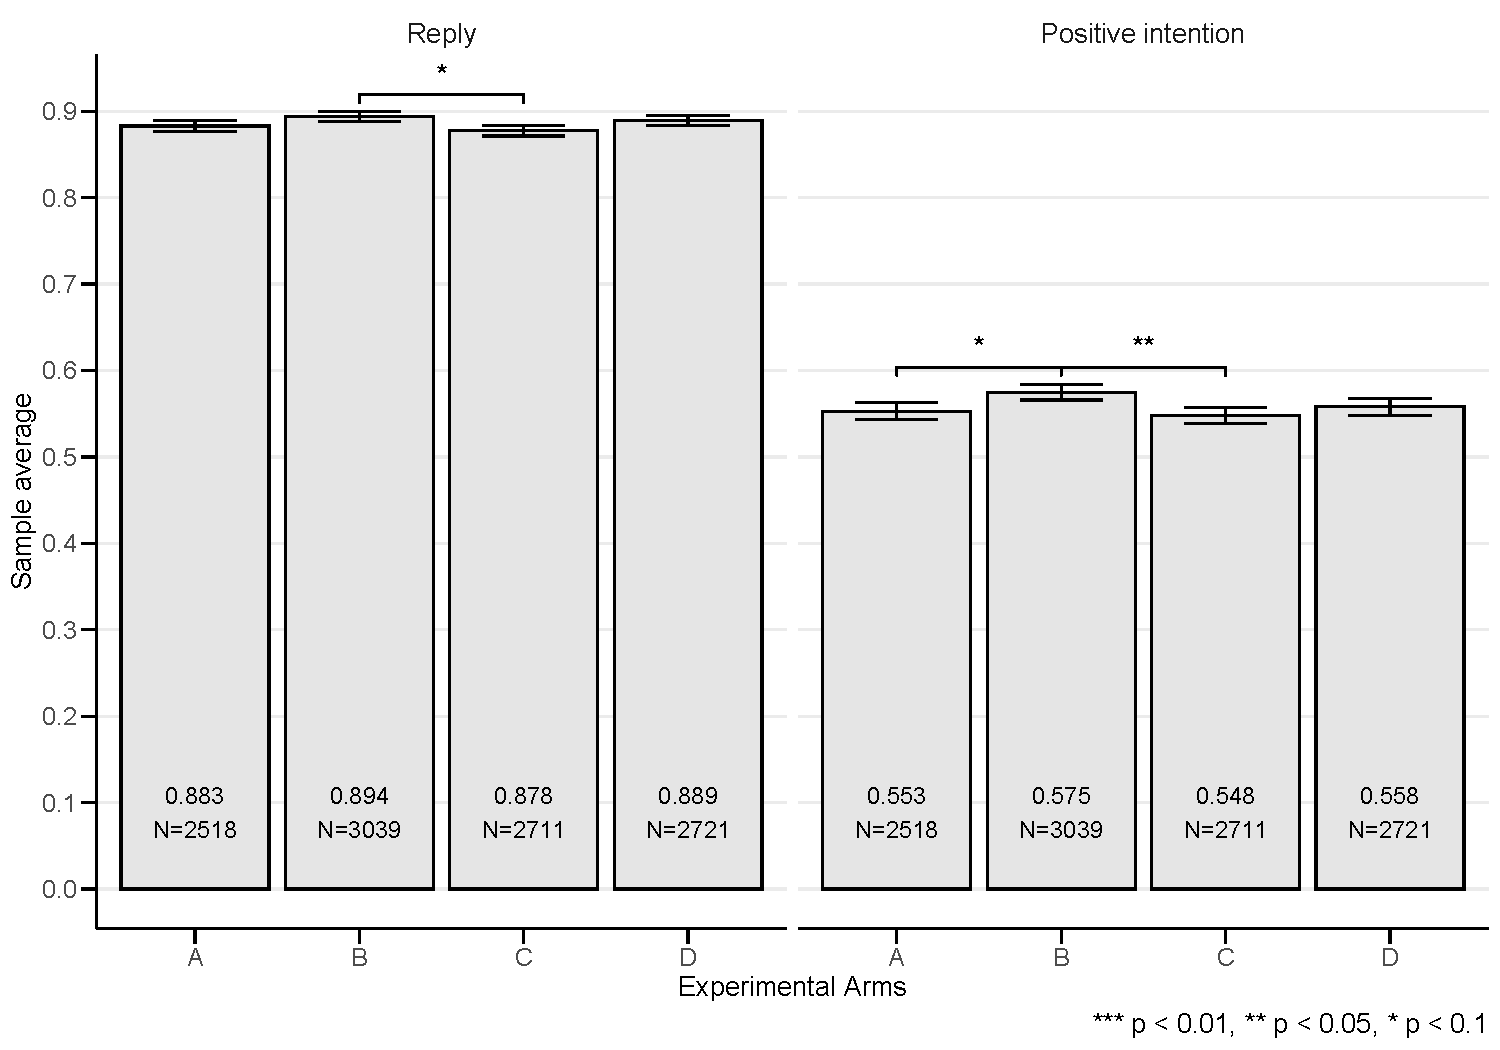
\includegraphics[width=0.75\linewidth]{C:/Users/katoo/Desktop/JMDP/RCT-Nudge/docs/slide/220818解析途中報告_files/figure-beamer/ttest-reply-1} \end{center}
\end{frame}

\begin{frame}{Linear Probability Model}
\protect\hypertarget{linear-probability-model}{}
\(m\)月の第\(w\)週に適合通知を受け取った個人\(i\)について、

\[
  Y_{imw} =
  \beta_1 \cdot \text{B}_{mw} + \beta_2 \cdot \text{C}_{mw}
  + \beta_3 \cdot \text{D}_{mw}
  + X'_i \gamma + \lambda_m + \theta_w + u_{imw}
\]

\begin{itemize}
\tightlist
\item
  \(X_i\)は性別・年齢・居住する都道府県・コーディネーション回数
\item
  \(\lambda_m\)と\(\theta_w\)は週・月の固定効果
\item
  \(\beta_1 = \beta_2\)、\(\beta_1 = \beta_3\)、\(\beta_2 = \beta_3\)の帰無仮説に対する
  F検定を実施
\end{itemize}
\end{frame}

\begin{frame}{Linear Probability Model of Reply}
\protect\hypertarget{linear-probability-model-of-reply}{}
\begin{table}
\centering
\fontsize{9}{11}\selectfont
\begin{tabular}[t]{l>{\centering\arraybackslash}p{6em}>{\centering\arraybackslash}p{6em}>{\centering\arraybackslash}p{6em}>{\centering\arraybackslash}p{6em}>{\centering\arraybackslash}p{6em}}
\toprule
\multicolumn{2}{c}{ } & \multicolumn{4}{c}{Reply within specific day} \\
\cmidrule(l{3pt}r{3pt}){3-6}
\multicolumn{1}{c}{ } & \multicolumn{1}{c}{Reply} & \multicolumn{1}{c}{5 days} & \multicolumn{1}{c}{10 days} & \multicolumn{1}{c}{20 days} & \multicolumn{1}{c}{30 days} \\
\cmidrule(l{3pt}r{3pt}){2-2} \cmidrule(l{3pt}r{3pt}){3-3} \cmidrule(l{3pt}r{3pt}){4-4} \cmidrule(l{3pt}r{3pt}){5-5} \cmidrule(l{3pt}r{3pt}){6-6}
  & (1) & (2) & (3) & (4) & (5)\\
\midrule
B & \num{0.013}** & \num{0.006} & \num{-0.044}*** & \num{0.013} & \num{0.015}**\\
 & (\num{0.006}) & (\num{0.008}) & (\num{0.014}) & (\num{0.009}) & (\num{0.007})\\
C & \num{0.002} & \num{0.002} & \num{0.002} & \num{0.007} & \num{0.004}\\
 & (\num{0.005}) & (\num{0.007}) & (\num{0.015}) & (\num{0.007}) & (\num{0.006})\\
D & \num{0.006} & \num{0.013} & \num{-0.028}* & \num{0.018}** & \num{0.007}\\
 & (\num{0.005}) & (\num{0.009}) & (\num{0.014}) & (\num{0.007}) & (\num{0.005})\\
\midrule
Num.Obs. & \num{11093} & \num{11093} & \num{11093} & \num{11093} & \num{11093}\\
\addlinespace[0.3em]
\multicolumn{6}{l}{\textit{F-tests, p-value}}\\
\hspace{1em}B = C & \num{0.015} & \num{0.590} & \num{0.004} & \num{0.282} & \num{0.028}\\
\hspace{1em}B = D & \num{0.233} & \num{0.447} & \num{0.259} & \num{0.474} & \num{0.135}\\
\hspace{1em}C = D & \num{0.277} & \num{0.148} & \num{0.064} & \num{0.022} & \num{0.463}\\
\bottomrule
\multicolumn{6}{l}{\rule{0pt}{1em}* p $<$ 0.1, ** p $<$ 0.05, *** p $<$ 0.01}\\
\end{tabular}
\end{table}
\end{frame}

\begin{frame}{Linear Probability Model of Intention}
\protect\hypertarget{linear-probability-model-of-intention}{}
\begin{table}
\centering
\fontsize{9}{11}\selectfont
\begin{tabular}[t]{l>{\centering\arraybackslash}p{6em}>{\centering\arraybackslash}p{6em}>{\centering\arraybackslash}p{6em}>{\centering\arraybackslash}p{6em}>{\centering\arraybackslash}p{6em}}
\toprule
\multicolumn{2}{c}{ } & \multicolumn{4}{c}{Intention with reply within specific day} \\
\cmidrule(l{3pt}r{3pt}){3-6}
\multicolumn{1}{c}{ } & \multicolumn{1}{c}{Intention} & \multicolumn{1}{c}{5 days} & \multicolumn{1}{c}{10 days} & \multicolumn{1}{c}{20 days} & \multicolumn{1}{c}{30 days} \\
\cmidrule(l{3pt}r{3pt}){2-2} \cmidrule(l{3pt}r{3pt}){3-3} \cmidrule(l{3pt}r{3pt}){4-4} \cmidrule(l{3pt}r{3pt}){5-5} \cmidrule(l{3pt}r{3pt}){6-6}
  & (1) & (2) & (3) & (4) & (5)\\
\midrule
B & \num{0.020} & \num{0.014} & \num{-0.017}* & \num{0.021} & \num{0.021}\\
 & (\num{0.012}) & (\num{0.009}) & (\num{0.009}) & (\num{0.013}) & (\num{0.012})\\
C & \num{-0.004} & \num{0.003} & \num{0.004} & \num{-0.003} & \num{-0.004}\\
 & (\num{0.011}) & (\num{0.009}) & (\num{0.014}) & (\num{0.011}) & (\num{0.011})\\
D & \num{0.007} & \num{0.015} & \num{-0.015} & \num{0.016} & \num{0.009}\\
 & (\num{0.010}) & (\num{0.009}) & (\num{0.010}) & (\num{0.011}) & (\num{0.010})\\
\midrule
Num.Obs. & \num{11093} & \num{11093} & \num{11093} & \num{11093} & \num{11093}\\
\addlinespace[0.3em]
\multicolumn{6}{l}{\textit{F-tests, p-value}}\\
\hspace{1em}B = C & \num{0.007} & \num{0.187} & \num{0.147} & \num{0.009} & \num{0.004}\\
\hspace{1em}B = D & \num{0.123} & \num{0.850} & \num{0.772} & \num{0.552} & \num{0.130}\\
\hspace{1em}C = D & \num{0.139} & \num{0.138} & \num{0.198} & \num{0.013} & \num{0.070}\\
\bottomrule
\multicolumn{6}{l}{\rule{0pt}{1em}* p $<$ 0.1, ** p $<$ 0.05, *** p $<$ 0.01}\\
\end{tabular}
\end{table}
\end{frame}

\begin{frame}{Heterogenous Effect on Reply by Gender x Age}
\protect\hypertarget{heterogenous-effect-on-reply-by-gender-x-age}{}
性別と年齢(30歳以下どうか)でサンプルを分割して、返信と意向の効果を推定する
\end{frame}

\begin{frame}{Heterogenity by Gender x Age: Message B (1)}
\protect\hypertarget{heterogenity-by-gender-x-age-message-b-1}{}
\begin{center}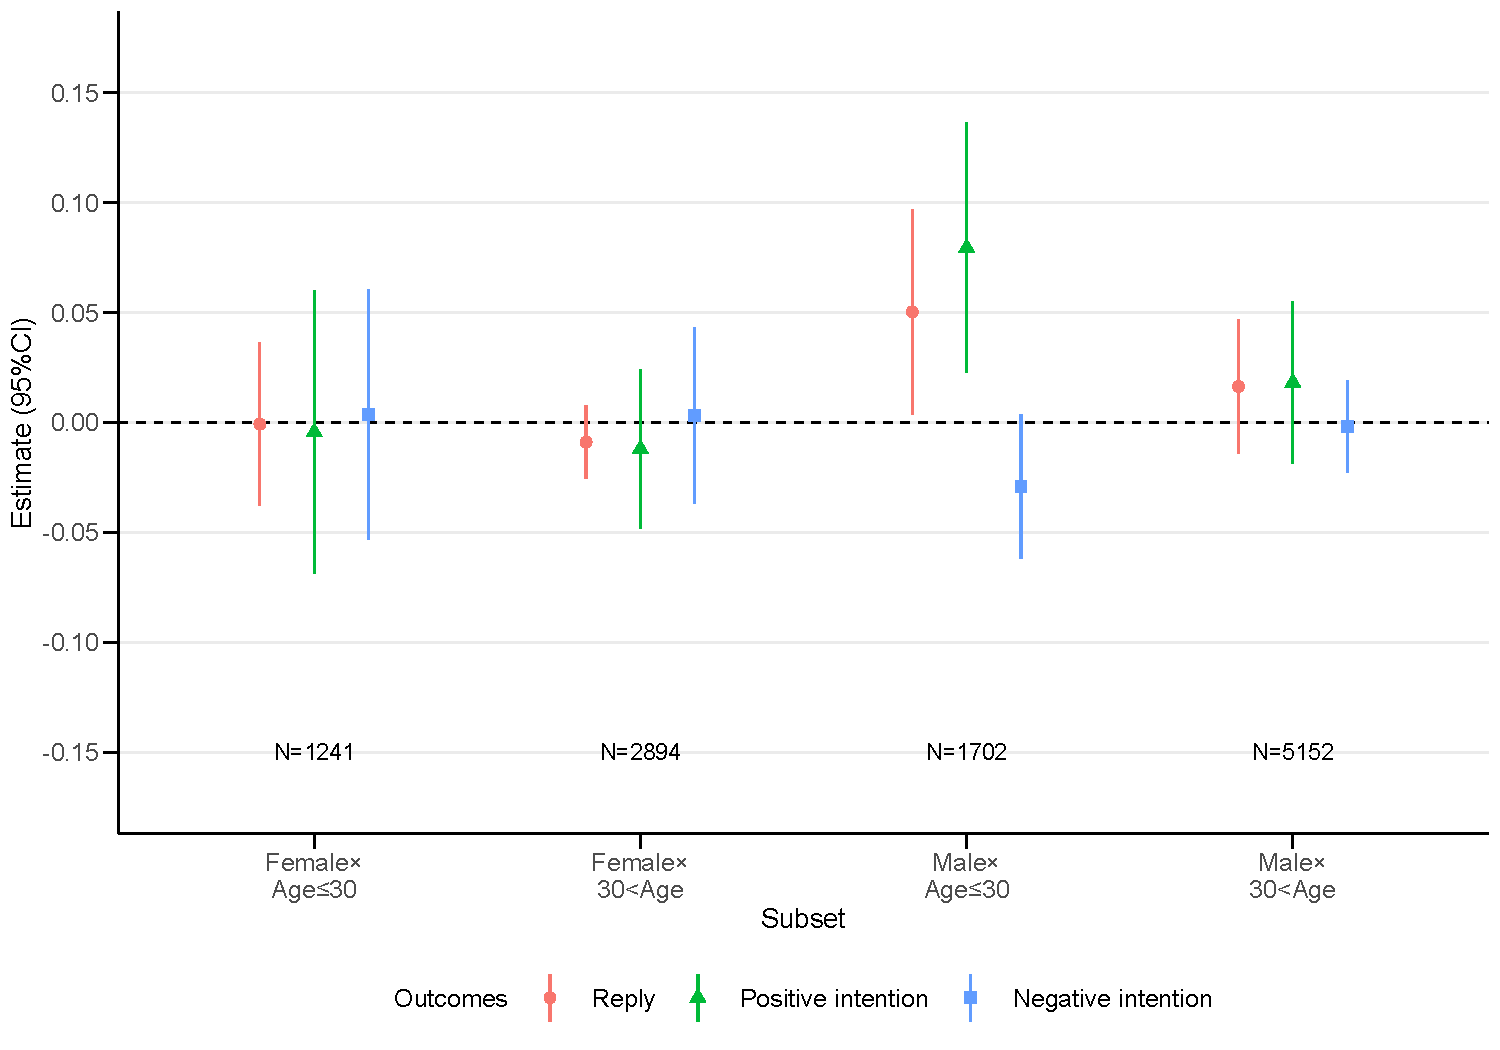
\includegraphics[width=0.75\linewidth]{C:/Users/katoo/Desktop/JMDP/RCT-Nudge/docs/slide/220818解析途中報告_files/figure-beamer/plotB-hetero-reply-gender-age-1} \end{center}
\end{frame}

\begin{frame}{Heterogenity by Gender x Age: Message C (1)}
\protect\hypertarget{heterogenity-by-gender-x-age-message-c-1}{}
\begin{center}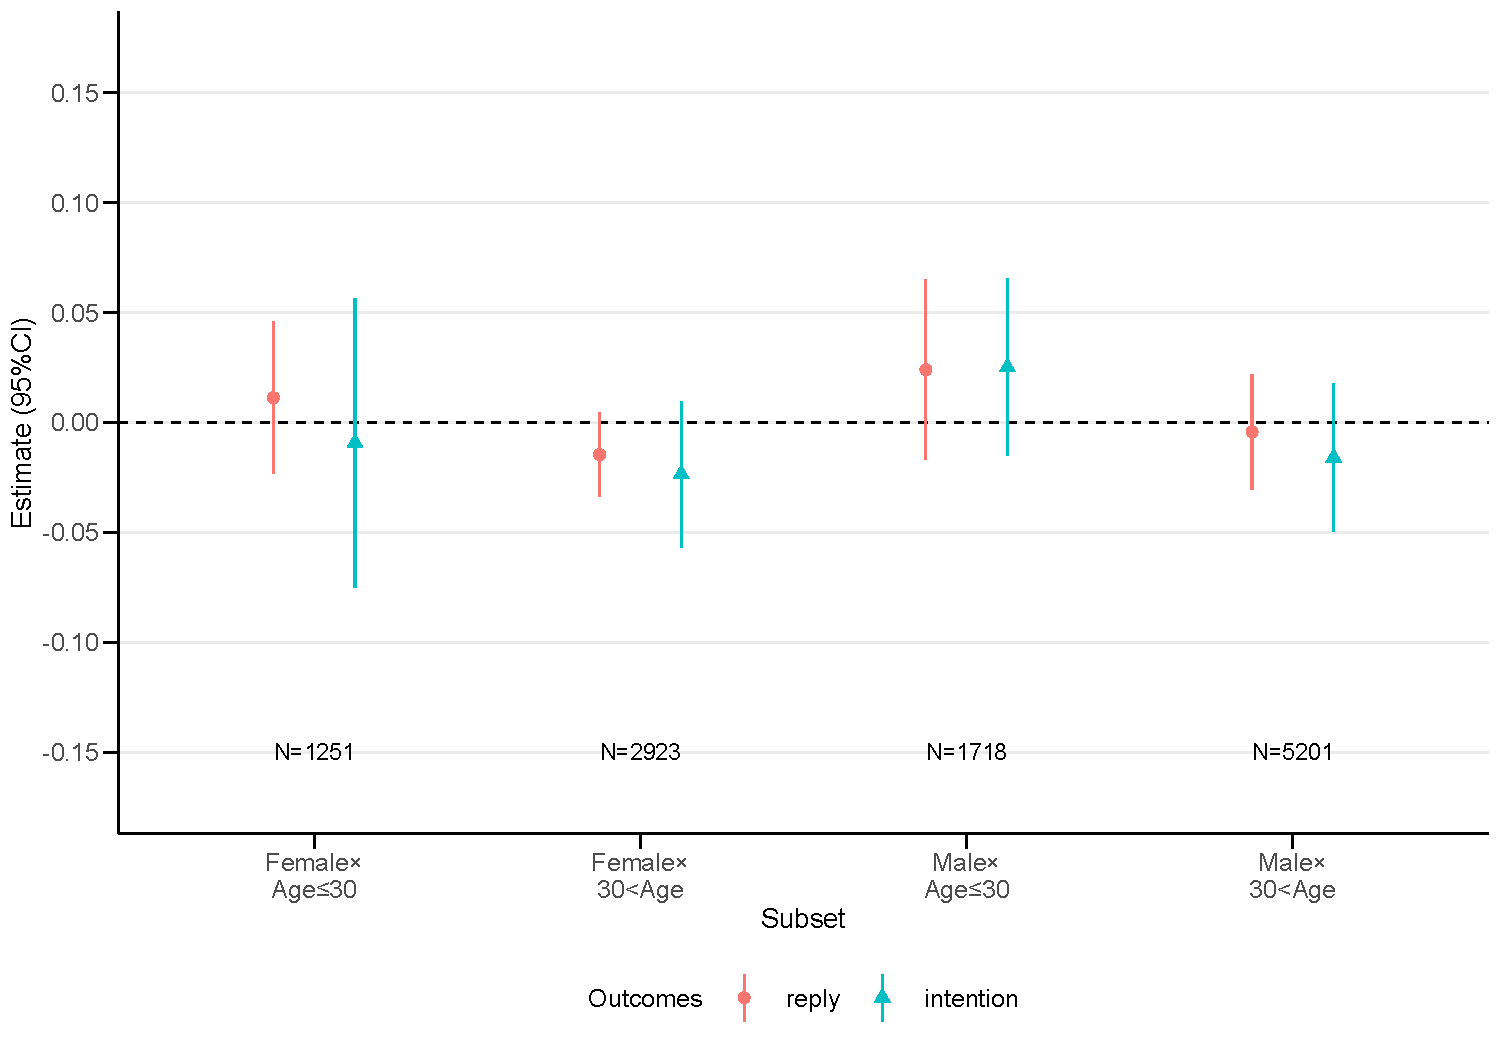
\includegraphics[width=0.75\linewidth]{C:/Users/katoo/Desktop/JMDP/RCT-Nudge/docs/slide/220818解析途中報告_files/figure-beamer/plotC-hetero-reply-gender-age-1} \end{center}
\end{frame}

\begin{frame}{Heterogenity by Gender x Age: Message D (1)}
\protect\hypertarget{heterogenity-by-gender-x-age-message-d-1}{}
\begin{center}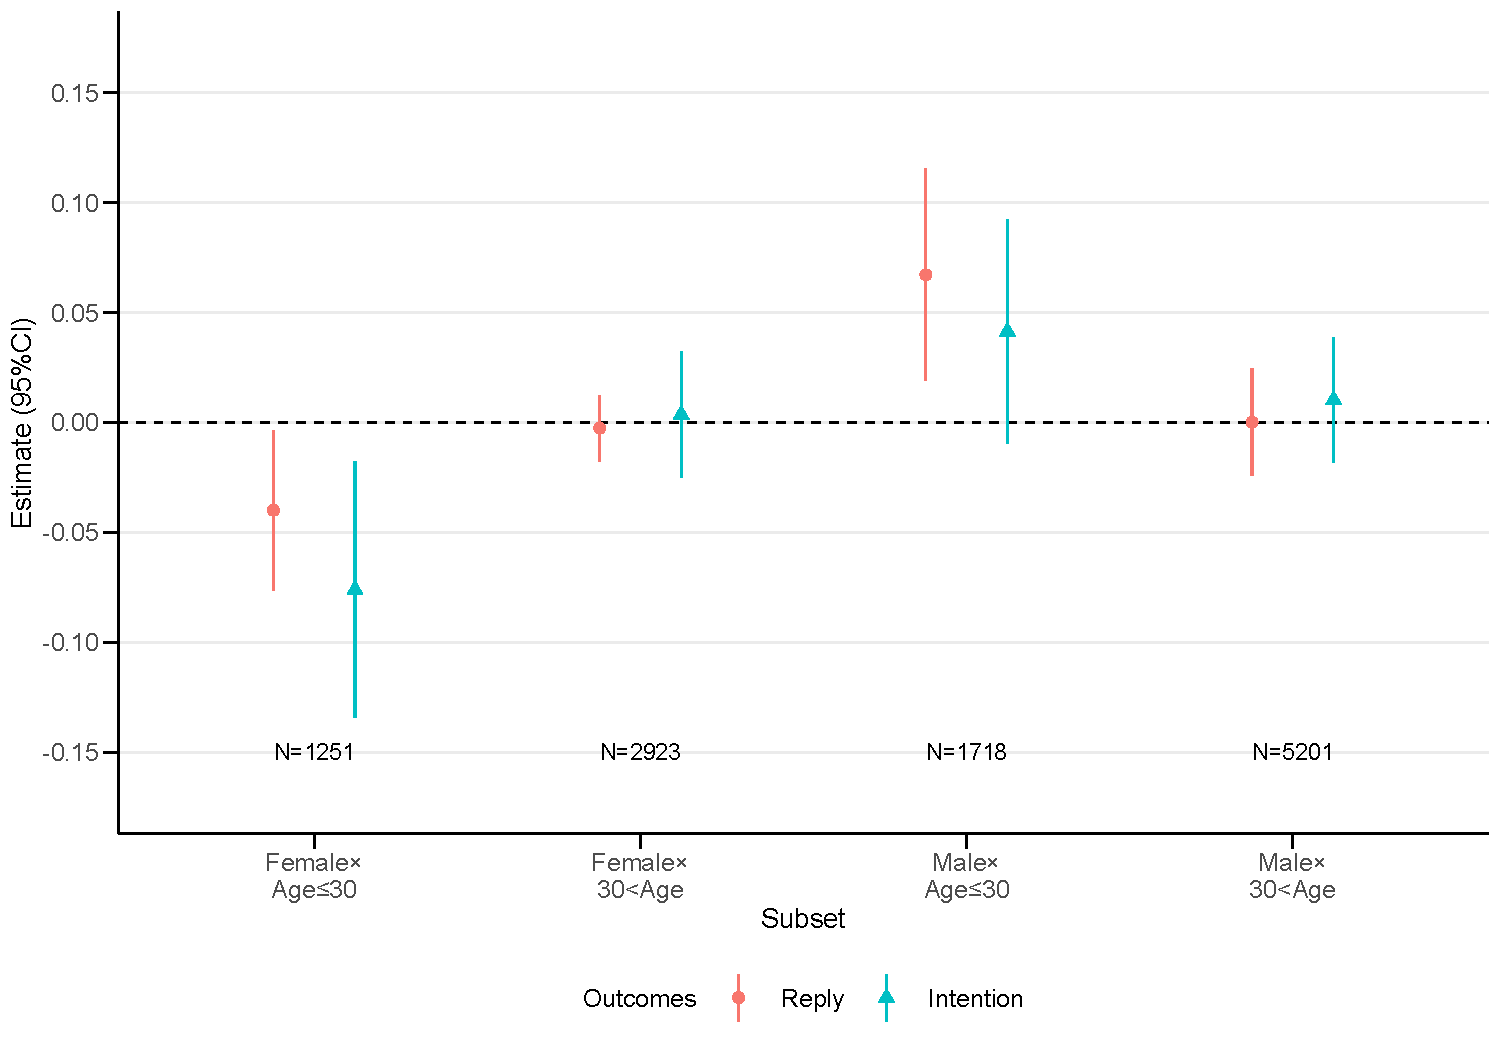
\includegraphics[width=0.75\linewidth]{C:/Users/katoo/Desktop/JMDP/RCT-Nudge/docs/slide/220818解析途中報告_files/figure-beamer/plotD-hetero-reply-gender-age-1} \end{center}
\end{frame}

\begin{frame}{Heterogenity by Gender x Age: Message B (2)}
\protect\hypertarget{heterogenity-by-gender-x-age-message-b-2}{}
\begin{center}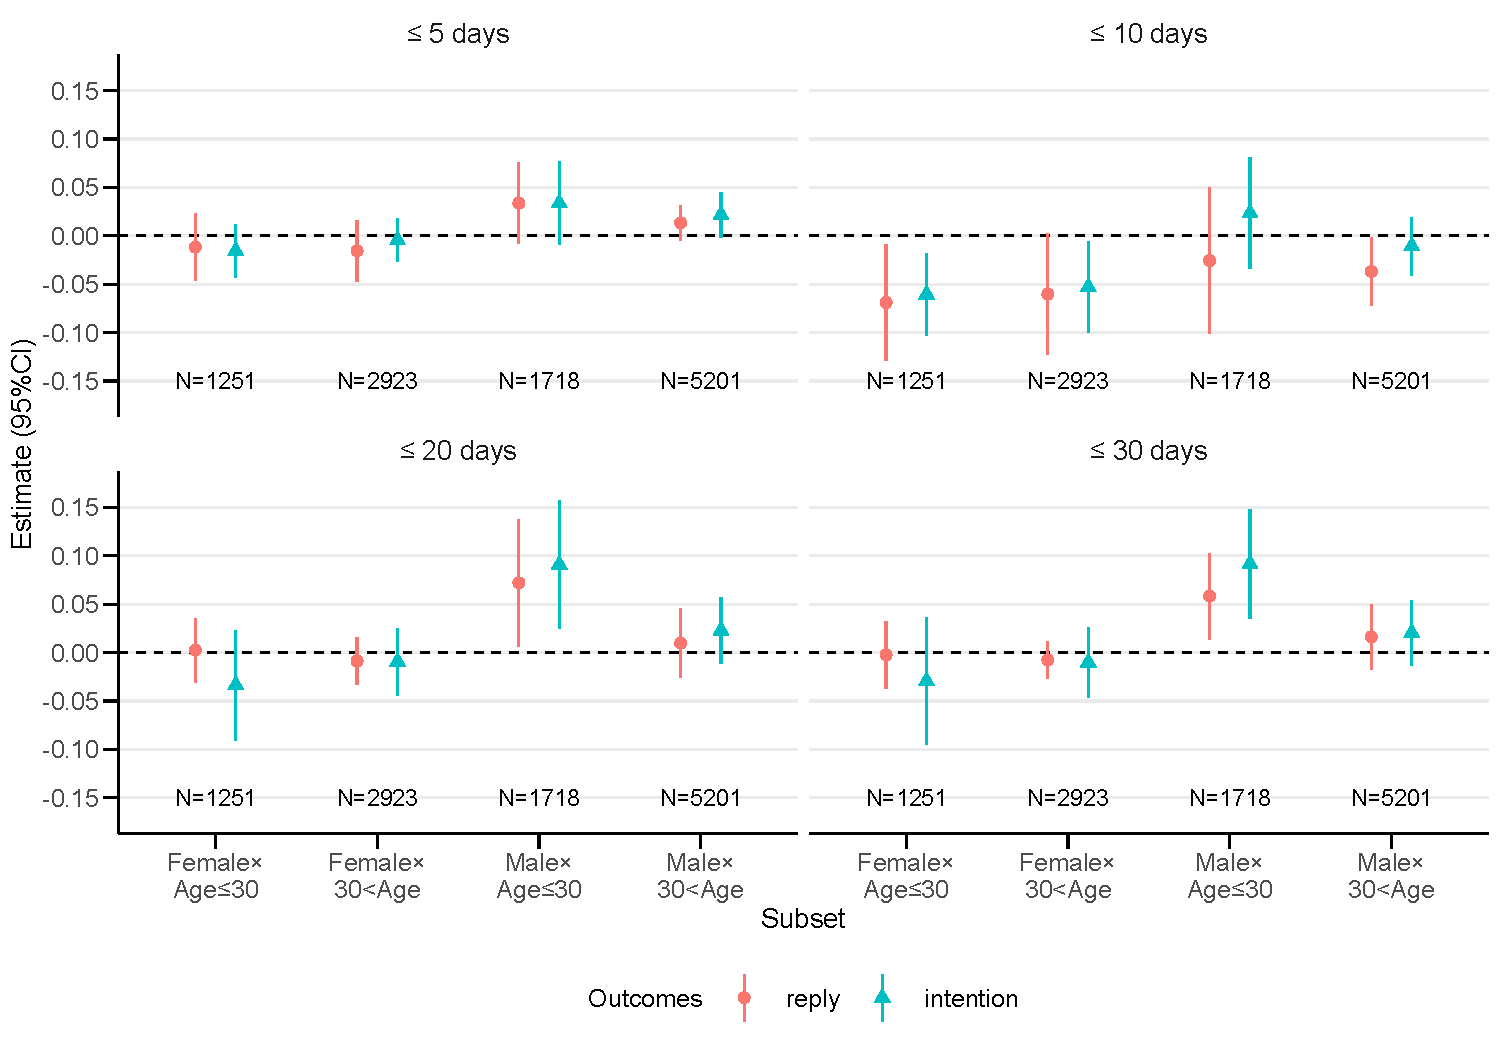
\includegraphics[width=0.75\linewidth]{C:/Users/katoo/Desktop/JMDP/RCT-Nudge/docs/slide/220818解析途中報告_files/figure-beamer/plotB-hetero-reply-within-gender-age-1} \end{center}
\end{frame}

\begin{frame}{Heterogenity by Gender x Age: Message C (2)}
\protect\hypertarget{heterogenity-by-gender-x-age-message-c-2}{}
\begin{center}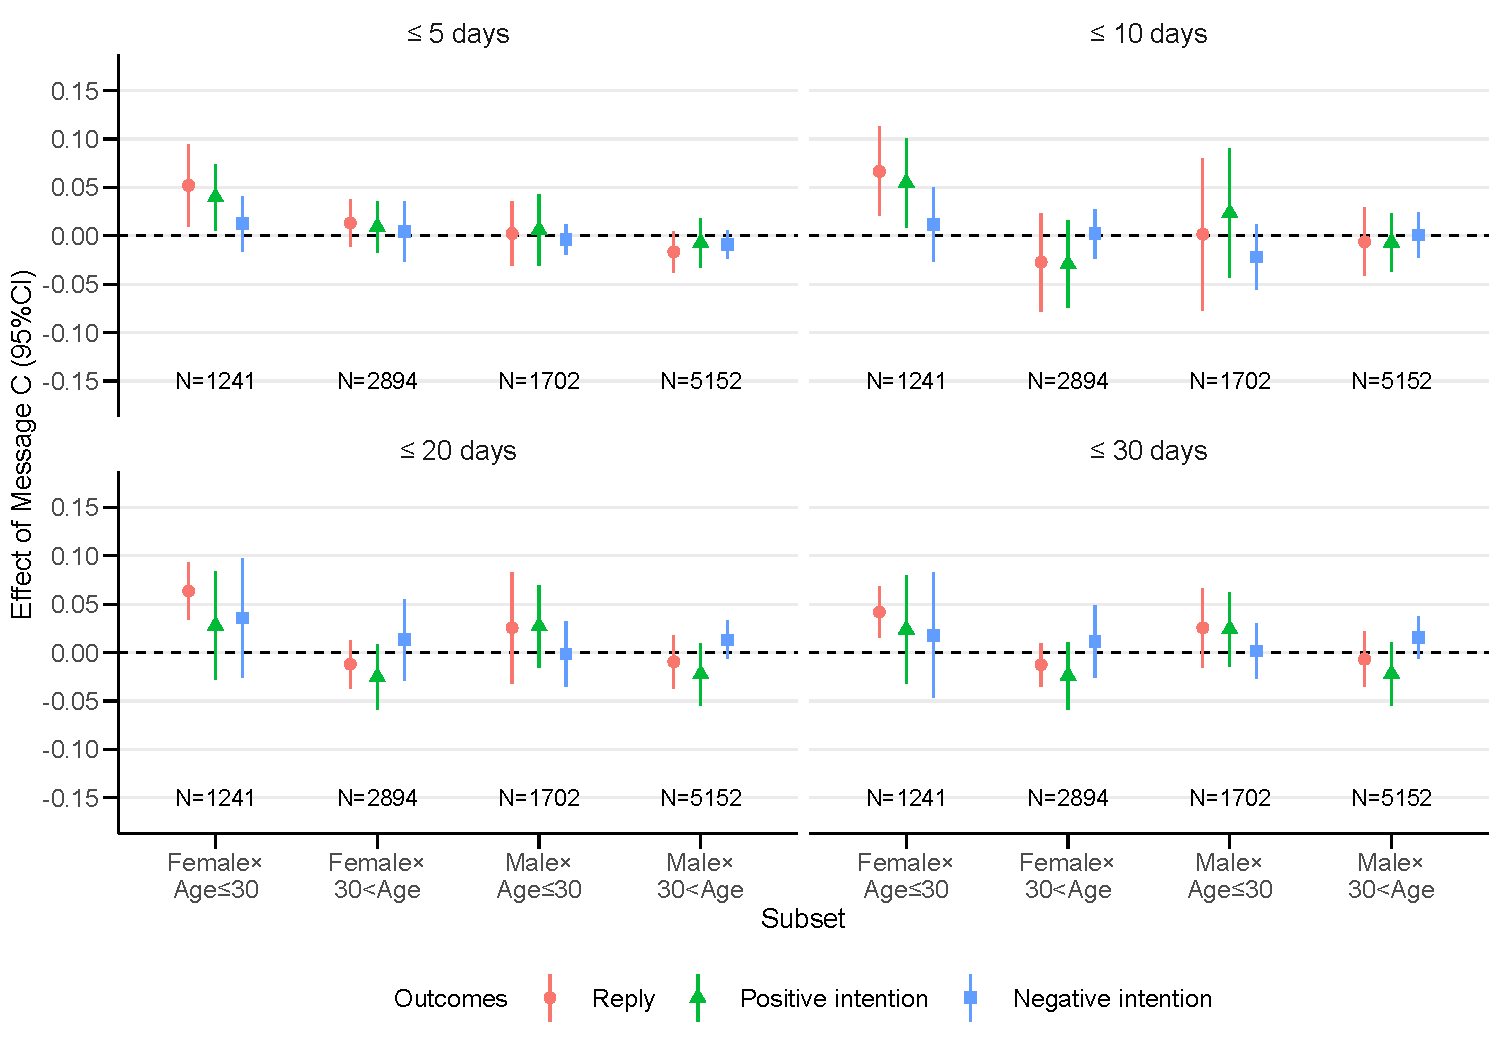
\includegraphics[width=0.75\linewidth]{C:/Users/katoo/Desktop/JMDP/RCT-Nudge/docs/slide/220818解析途中報告_files/figure-beamer/plotC-hetero-reply-within-gender-age-1} \end{center}
\end{frame}

\begin{frame}{Heterogenity by Gender x Age: Message D (2)}
\protect\hypertarget{heterogenity-by-gender-x-age-message-d-2}{}
\begin{center}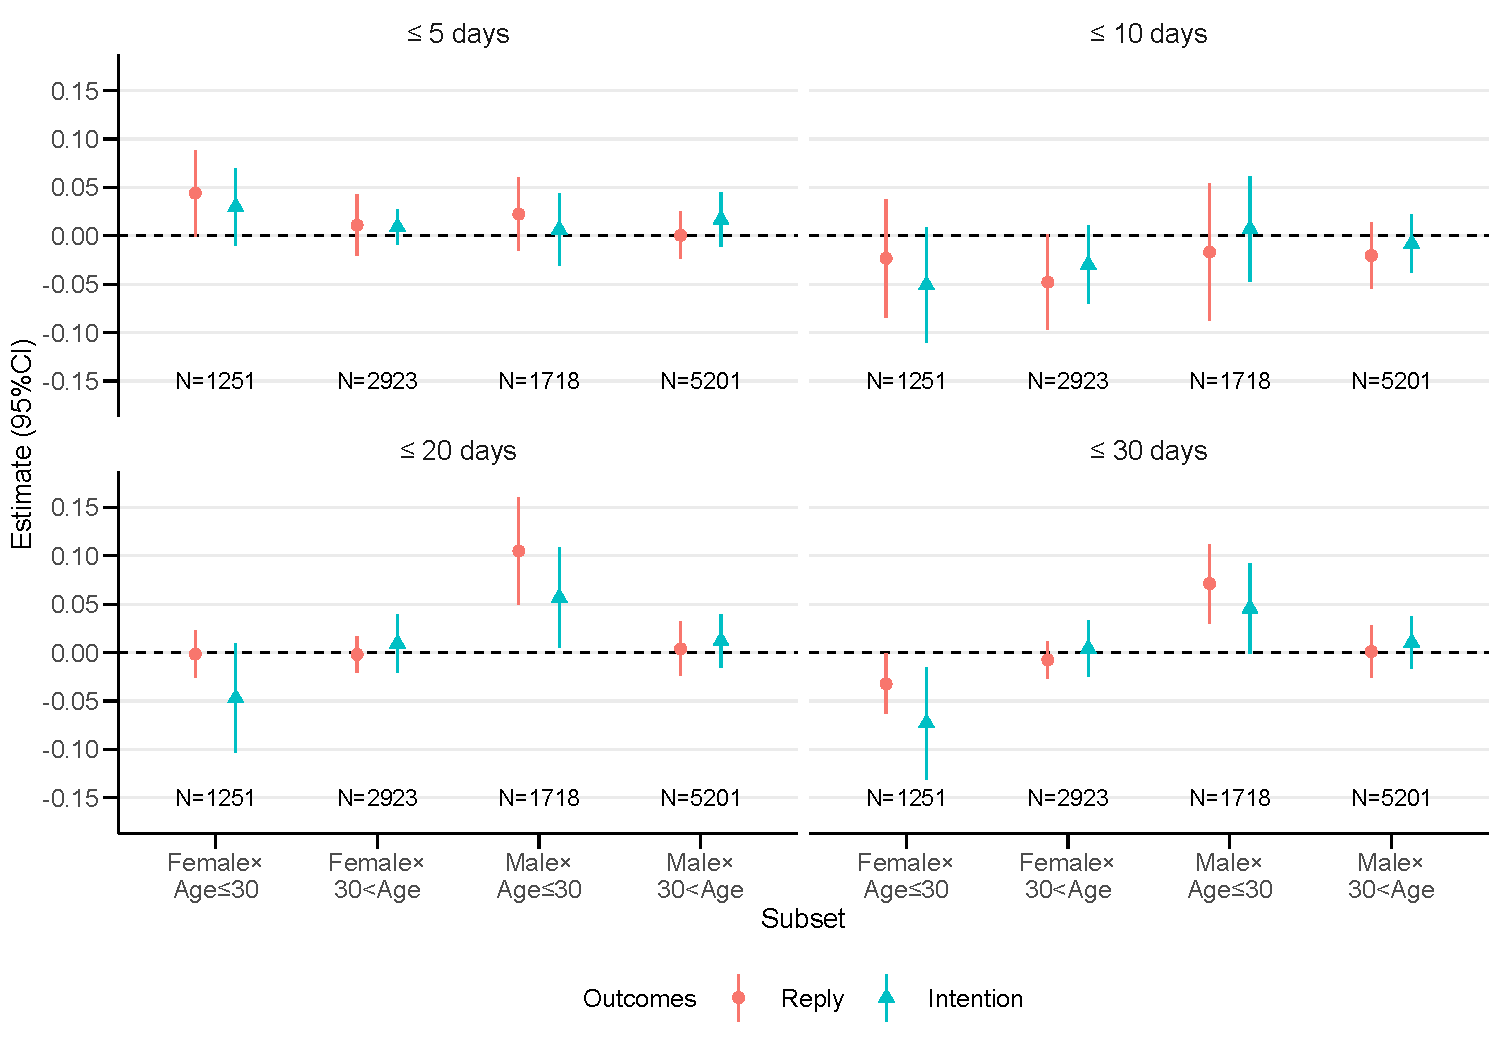
\includegraphics[width=0.75\linewidth]{C:/Users/katoo/Desktop/JMDP/RCT-Nudge/docs/slide/220818解析途中報告_files/figure-beamer/plotD-hetero-reply-within-gender-age-1} \end{center}
\end{frame}

\begin{frame}{Geographical Heterogenity}
\protect\hypertarget{geographical-heterogenity}{}
\begin{itemize}
\tightlist
\item
  都道府県ごとに10平方キロメートル当たりの病院数を計算し、
  0.5カ所以上ある地域とそうでない地域でサンプルを分割した

  \begin{itemize}
  \tightlist
  \item
    1カ所以上:東京・大阪
  \item
    1カ所未満:神奈川・愛知
  \end{itemize}
\item
  それぞれのサブサンプルで効果を推定する
\end{itemize}
\end{frame}

\begin{frame}{Heterogenity by Geography: Message B (1)}
\protect\hypertarget{heterogenity-by-geography-message-b-1}{}
\begin{center}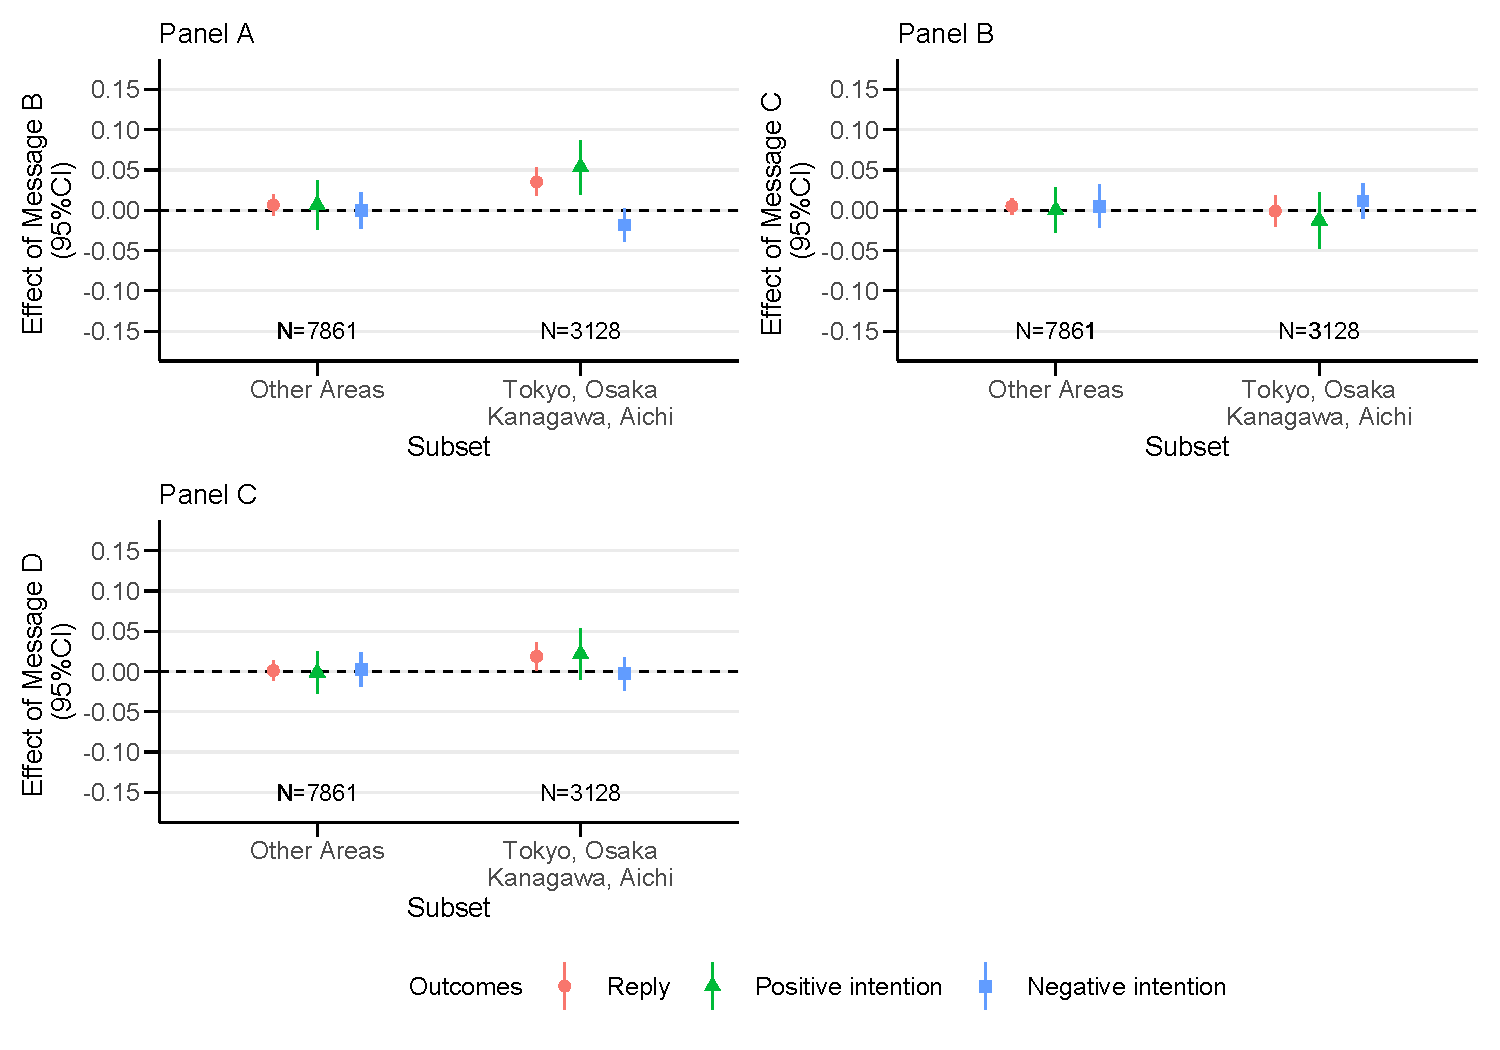
\includegraphics[width=0.75\linewidth]{C:/Users/katoo/Desktop/JMDP/RCT-Nudge/docs/slide/220818解析途中報告_files/figure-beamer/plotB-hetero-reply-geo-1} \end{center}
\end{frame}

\begin{frame}{Heterogenity by Geography: Message C (1)}
\protect\hypertarget{heterogenity-by-geography-message-c-1}{}
\begin{center}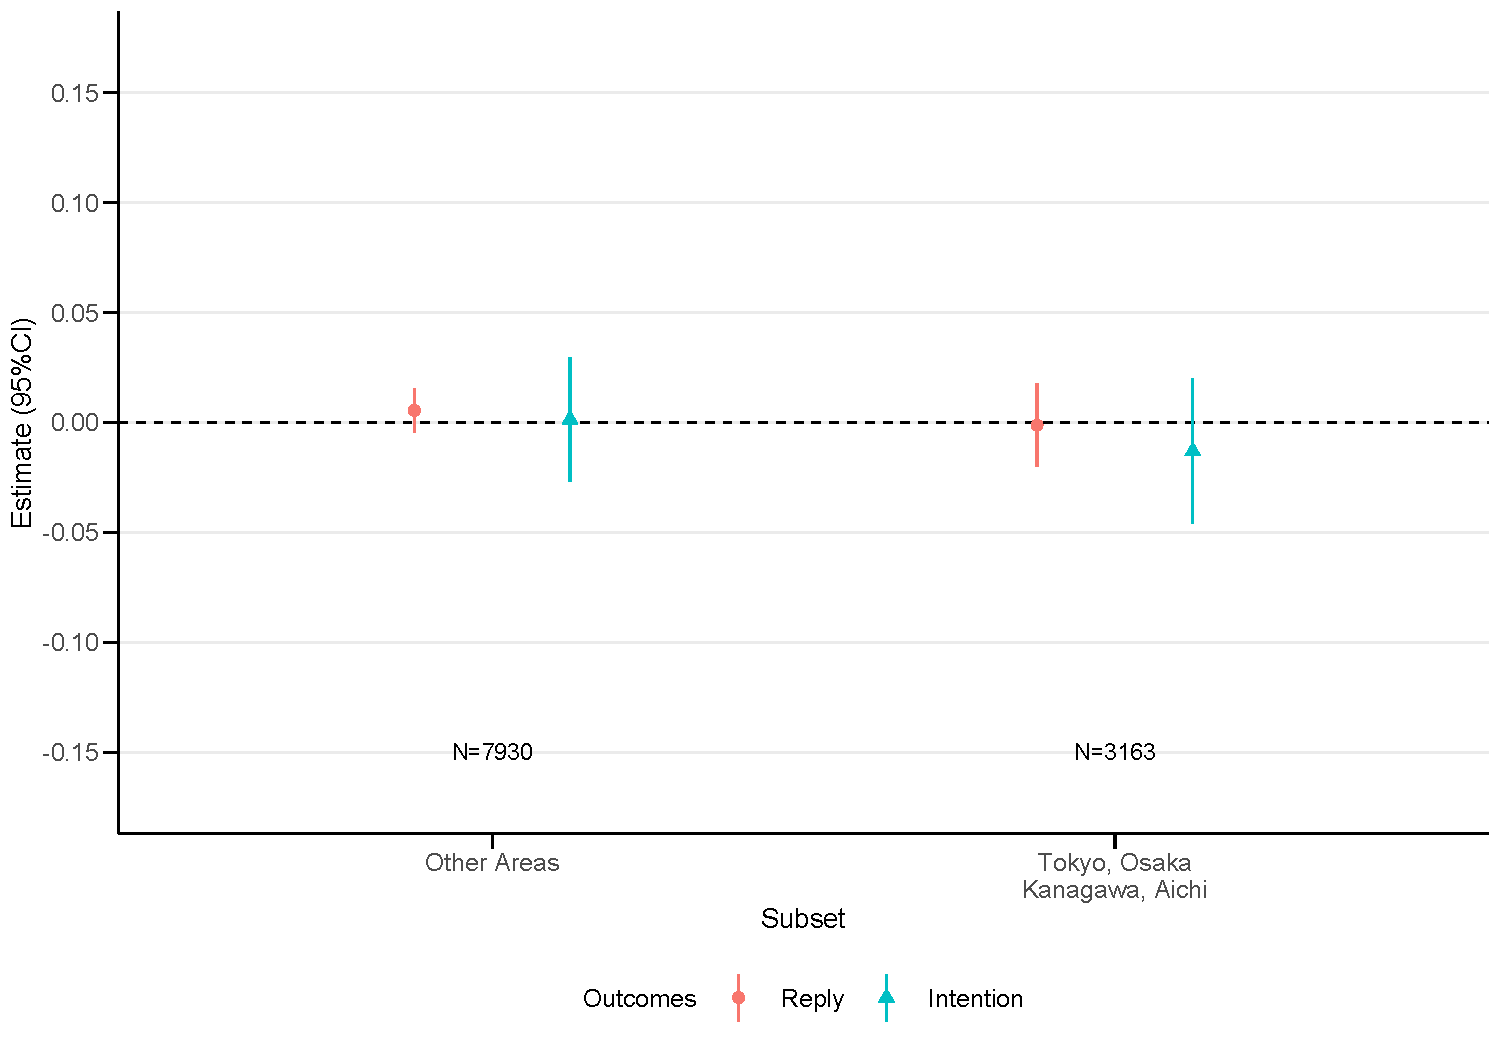
\includegraphics[width=0.75\linewidth]{C:/Users/katoo/Desktop/JMDP/RCT-Nudge/docs/slide/220818解析途中報告_files/figure-beamer/plotC-hetero-reply-geo-1} \end{center}
\end{frame}

\begin{frame}{Heterogenity by Geography: Message D (1)}
\protect\hypertarget{heterogenity-by-geography-message-d-1}{}
\begin{center}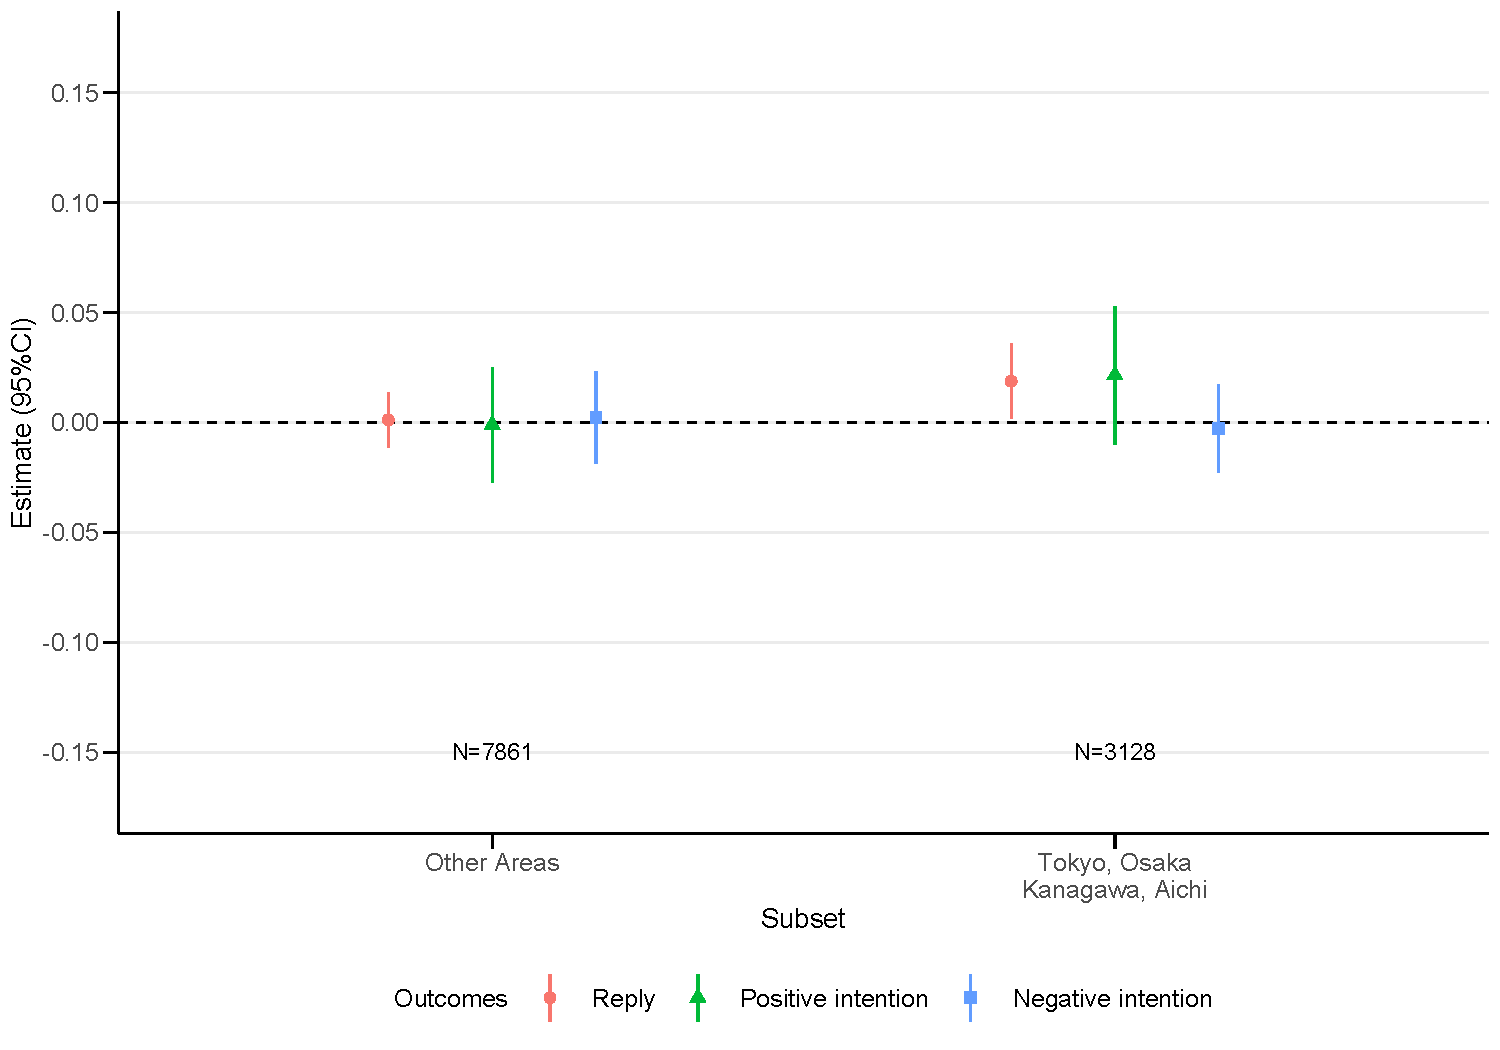
\includegraphics[width=0.75\linewidth]{C:/Users/katoo/Desktop/JMDP/RCT-Nudge/docs/slide/220818解析途中報告_files/figure-beamer/plotD-hetero-reply-geo-1} \end{center}
\end{frame}

\begin{frame}{Heterogenity by Geography: Message B (2)}
\protect\hypertarget{heterogenity-by-geography-message-b-2}{}
\begin{center}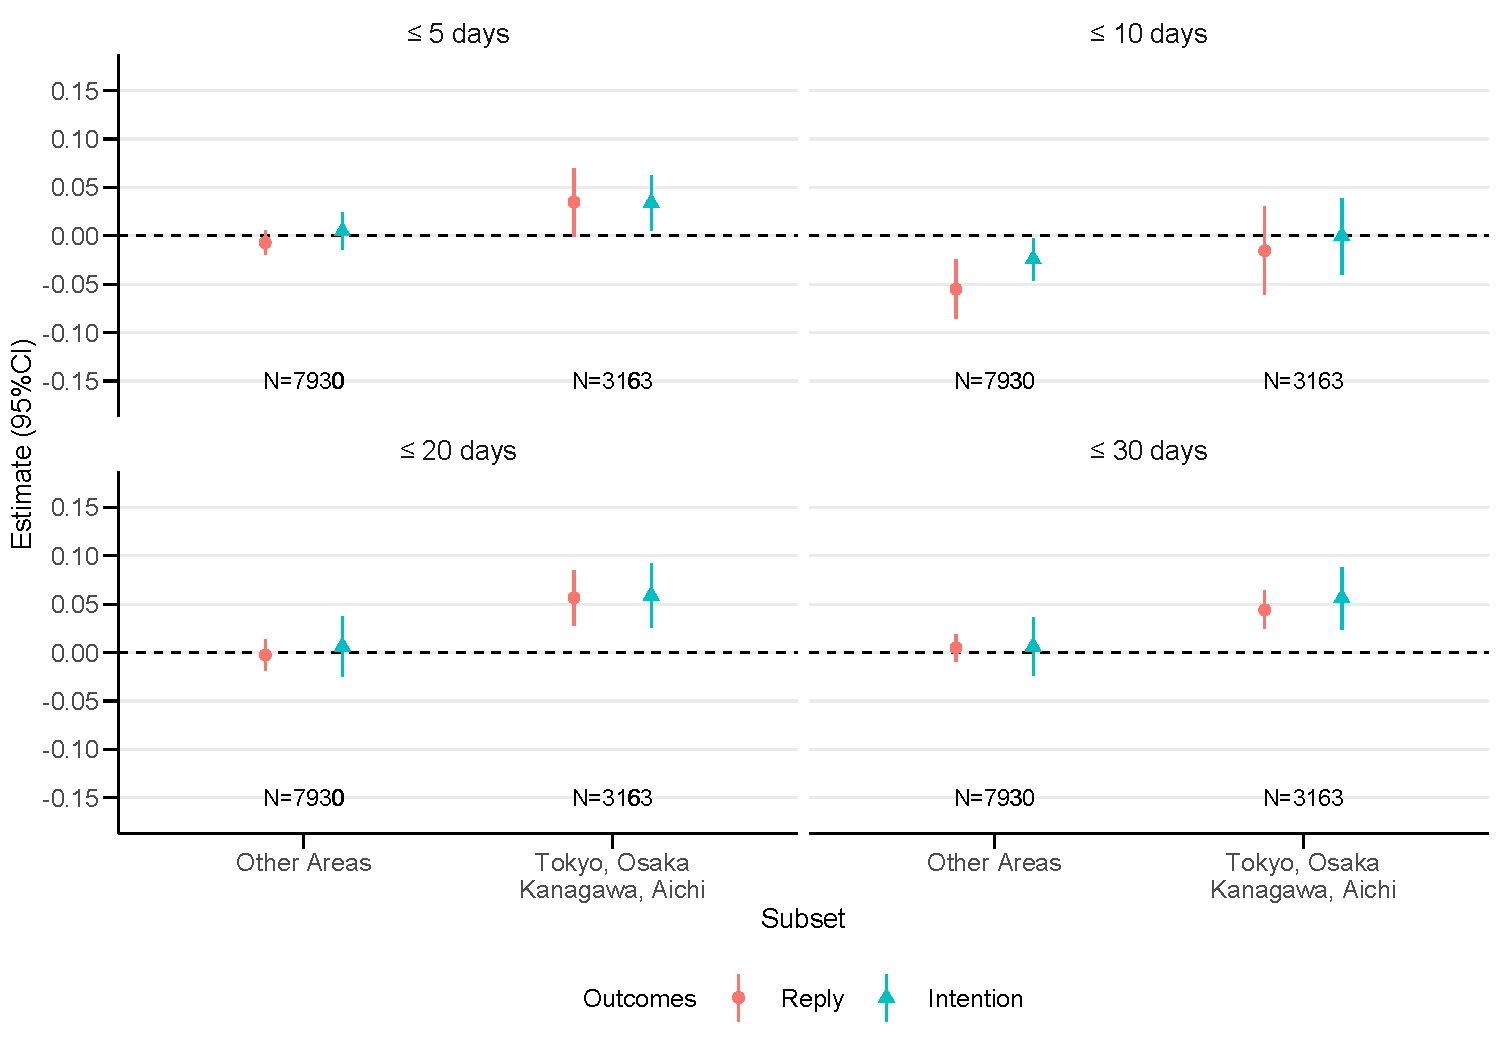
\includegraphics[width=0.75\linewidth]{C:/Users/katoo/Desktop/JMDP/RCT-Nudge/docs/slide/220818解析途中報告_files/figure-beamer/plotB-hetero-reply-within-geo-1} \end{center}
\end{frame}

\begin{frame}{Heterogenity by Geography: Message C (2)}
\protect\hypertarget{heterogenity-by-geography-message-c-2}{}
\begin{center}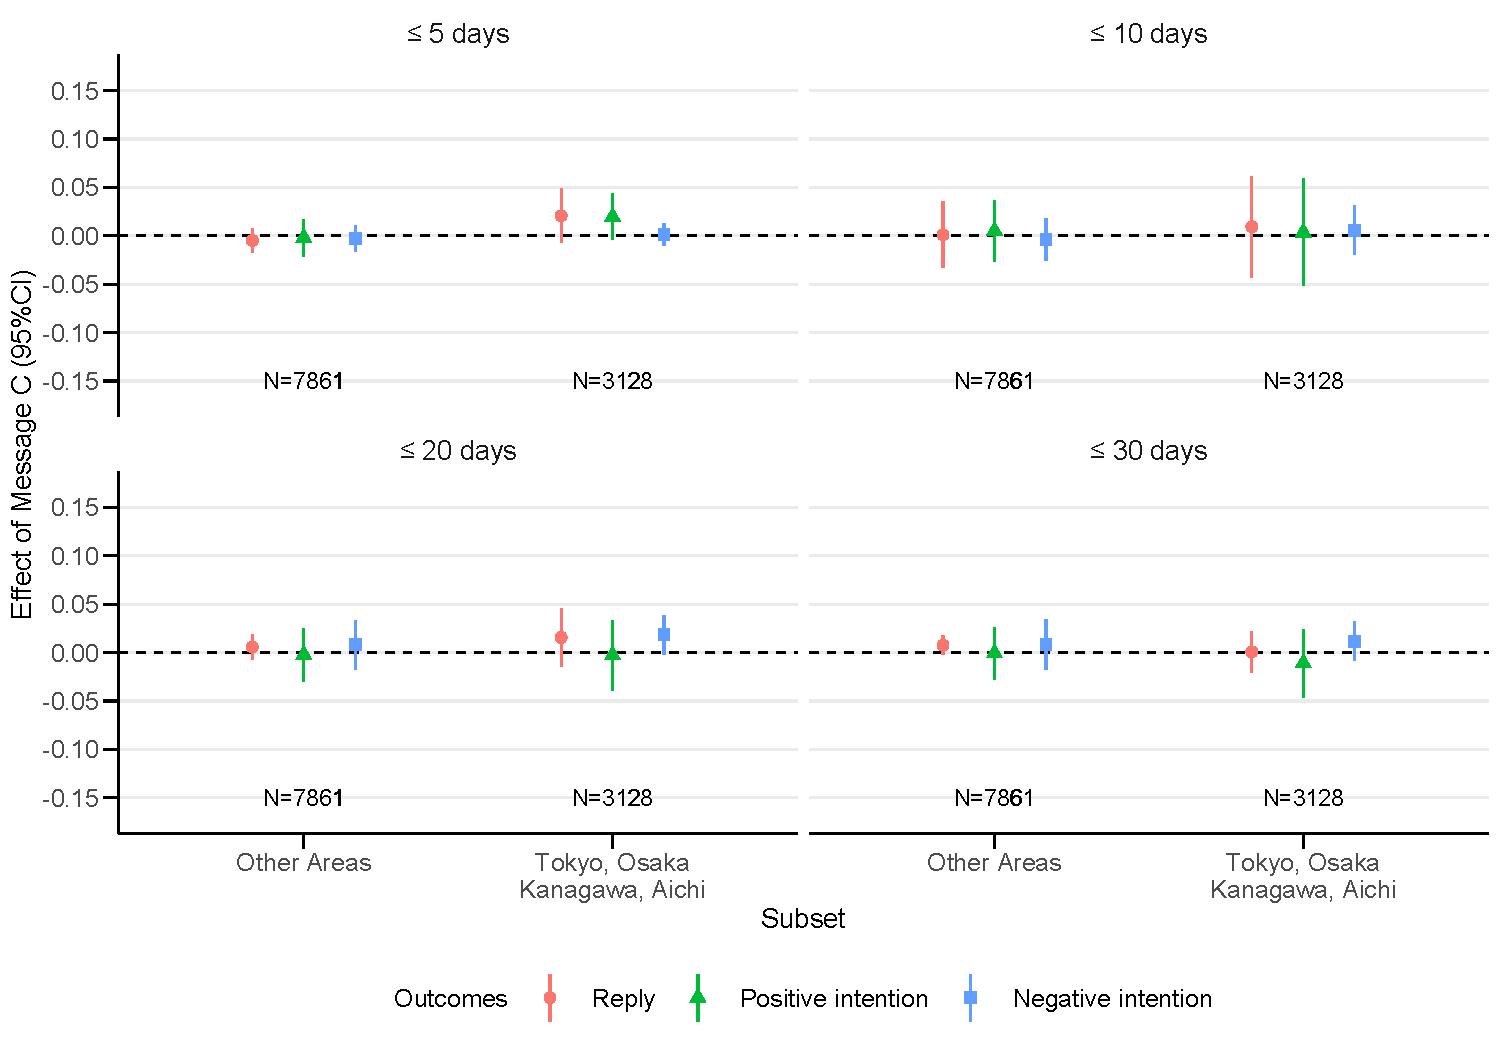
\includegraphics[width=0.75\linewidth]{C:/Users/katoo/Desktop/JMDP/RCT-Nudge/docs/slide/220818解析途中報告_files/figure-beamer/plotC-hetero-reply-within-geo-1} \end{center}
\end{frame}

\begin{frame}{Heterogenity by Geography: Message D (2)}
\protect\hypertarget{heterogenity-by-geography-message-d-2}{}
\begin{center}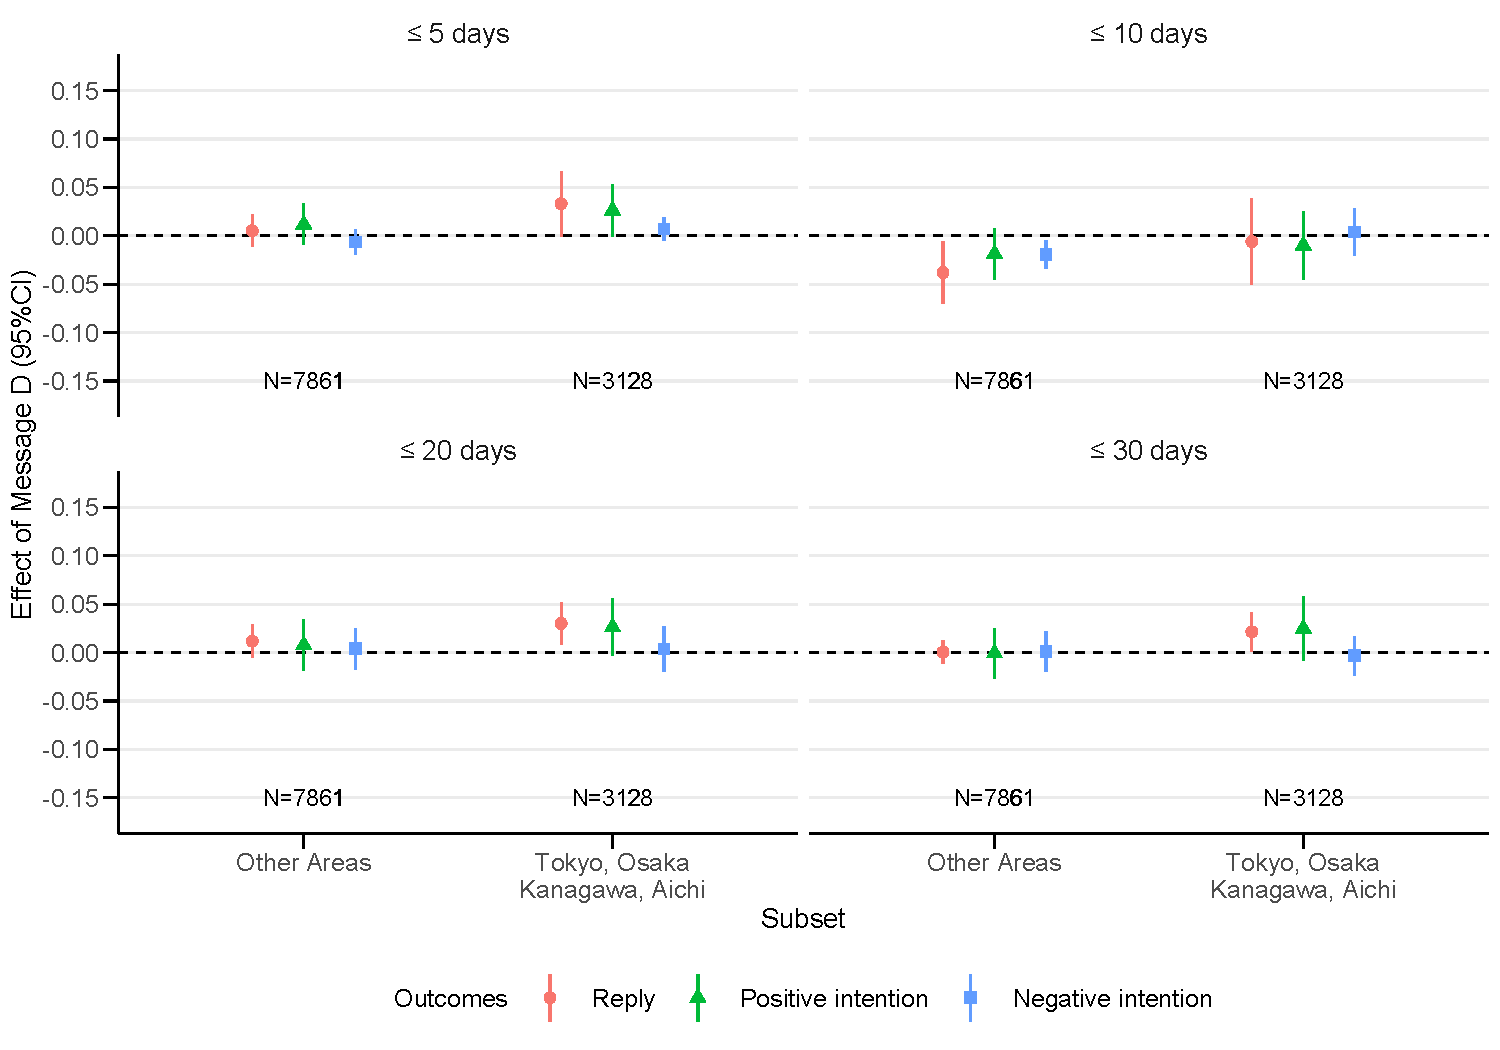
\includegraphics[width=0.75\linewidth]{C:/Users/katoo/Desktop/JMDP/RCT-Nudge/docs/slide/220818解析途中報告_files/figure-beamer/plotD-hetero-reply-within-geo-1} \end{center}
\end{frame}

\hypertarget{effect-on-process-after-reply}{%
\section{Effect on Process after Reply}\label{effect-on-process-after-reply}}

\begin{frame}{Difference-in-mean Test}
\protect\hypertarget{difference-in-mean-test}{}
\begin{center}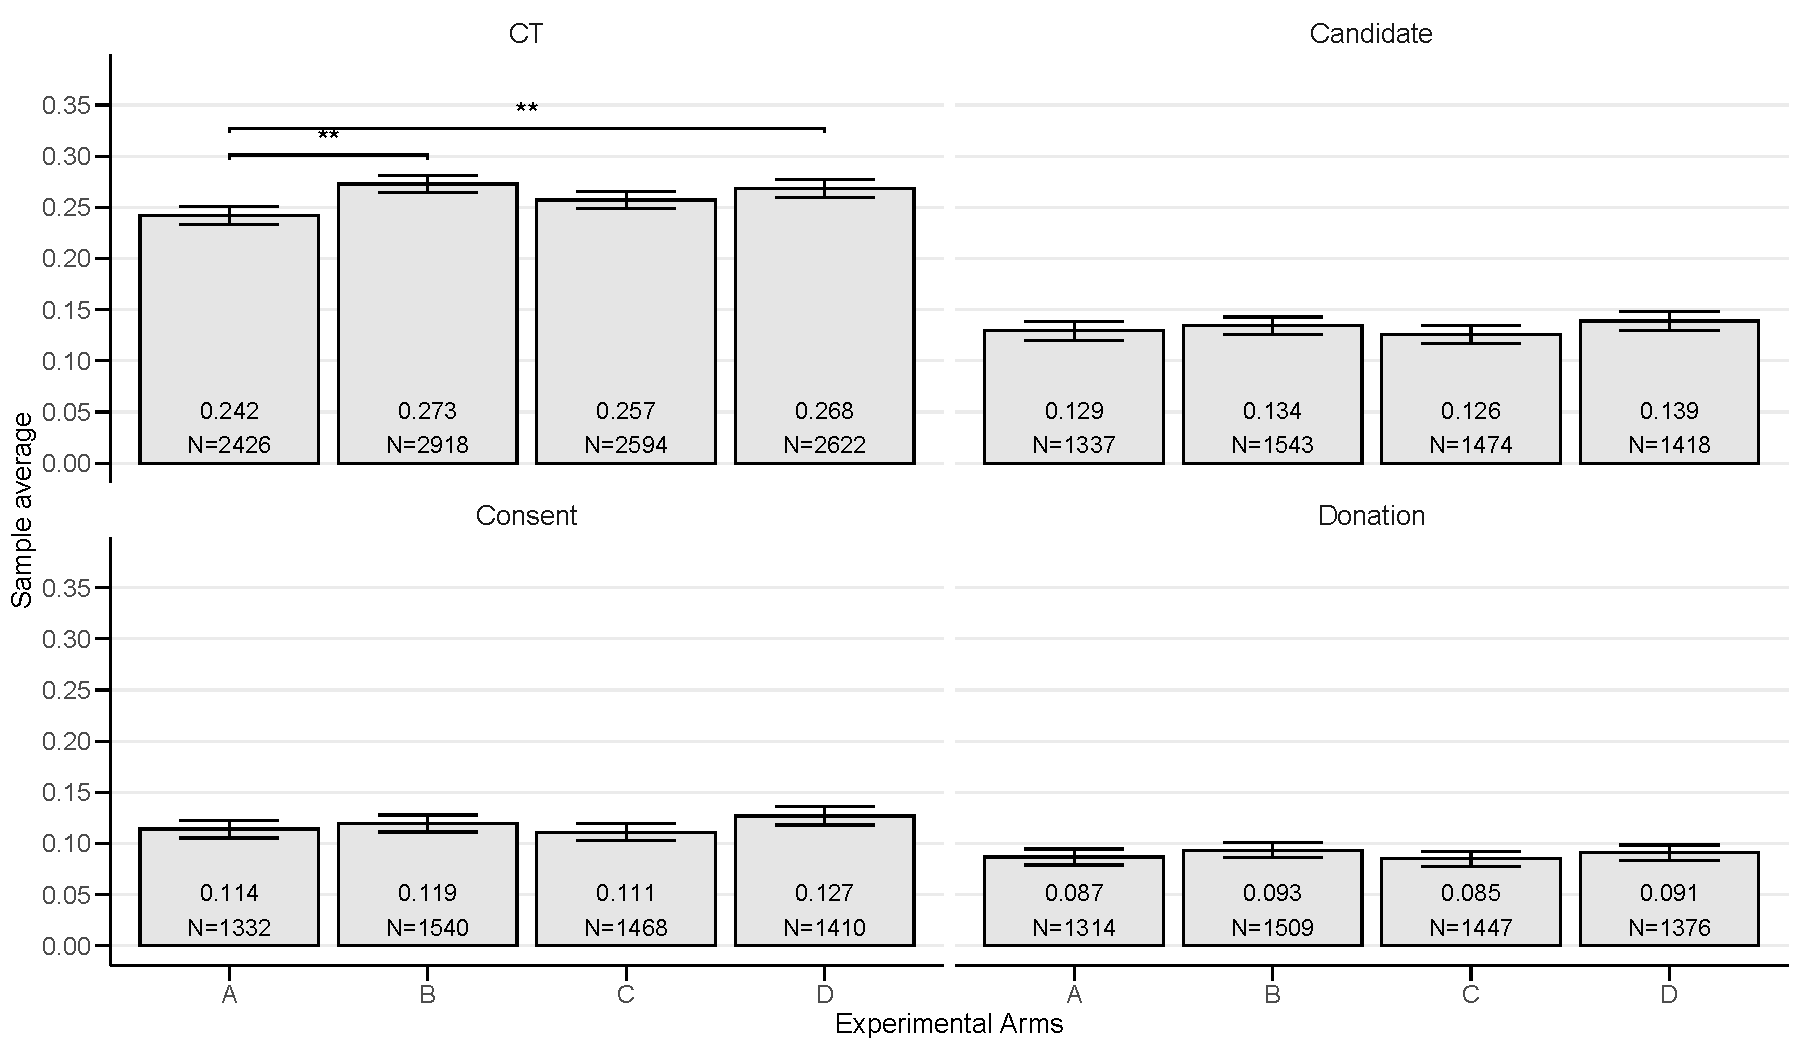
\includegraphics[width=0.75\linewidth]{C:/Users/katoo/Desktop/JMDP/RCT-Nudge/docs/slide/220818解析途中報告_files/figure-beamer/ttest-after-reply-1} \end{center}
\end{frame}

\begin{frame}{Linear Probability Model}
\protect\hypertarget{linear-probability-model-1}{}
\begin{table}
\centering
\fontsize{9}{11}\selectfont
\begin{tabular}[t]{l>{\centering\arraybackslash}p{5em}>{\centering\arraybackslash}p{5em}>{\centering\arraybackslash}p{5em}>{\centering\arraybackslash}p{5em}}
\toprule
\multicolumn{1}{c}{ } & \multicolumn{1}{c}{CT} & \multicolumn{1}{c}{Candidate} & \multicolumn{1}{c}{Consent} & \multicolumn{1}{c}{Donation} \\
\cmidrule(l{3pt}r{3pt}){2-2} \cmidrule(l{3pt}r{3pt}){3-3} \cmidrule(l{3pt}r{3pt}){4-4} \cmidrule(l{3pt}r{3pt}){5-5}
  & (1) & (2) & (3) & (4)\\
\midrule
B & \num{0.034}*** & \num{0.002} & \num{0.002} & \num{0.003}\\
 & (\num{0.009}) & (\num{0.009}) & (\num{0.007}) & (\num{0.007})\\
C & \num{0.015} & \num{-0.010} & \num{-0.009} & \num{-0.007}\\
 & (\num{0.010}) & (\num{0.009}) & (\num{0.007}) & (\num{0.008})\\
D & \num{0.032}*** & \num{0.008} & \num{0.011} & \num{0.002}\\
 & (\num{0.010}) & (\num{0.008}) & (\num{0.007}) & (\num{0.008})\\
\midrule
Num.Obs. & \num{10560} & \num{5772} & \num{5750} & \num{5646}\\
\addlinespace[0.3em]
\multicolumn{5}{l}{\textit{F-tests, p-value}}\\
\hspace{1em}B = C & \num{0.084} & \num{0.293} & \num{0.230} & \num{0.152}\\
\hspace{1em}B = D & \num{0.856} & \num{0.495} & \num{0.325} & \num{0.917}\\
\hspace{1em}C = D & \num{0.148} & \num{0.068} & \num{0.018} & \num{0.220}\\
\bottomrule
\multicolumn{5}{l}{\rule{0pt}{1em}* p $<$ 0.1, ** p $<$ 0.05, *** p $<$ 0.01}\\
\end{tabular}
\end{table}
\end{frame}

\begin{frame}{Heterogenous Effect by Gender and Age}
\protect\hypertarget{heterogenous-effect-by-gender-and-age}{}
\begin{itemize}
\tightlist
\item
  性別と年齢(30歳以下どうか)でサンプルを分割して、
  各サブサンプル内でメッセージの効果を推定した
\end{itemize}
\end{frame}

\begin{frame}{Heterogenity by Gender x Age: Message B}
\protect\hypertarget{heterogenity-by-gender-x-age-message-b}{}
\begin{center}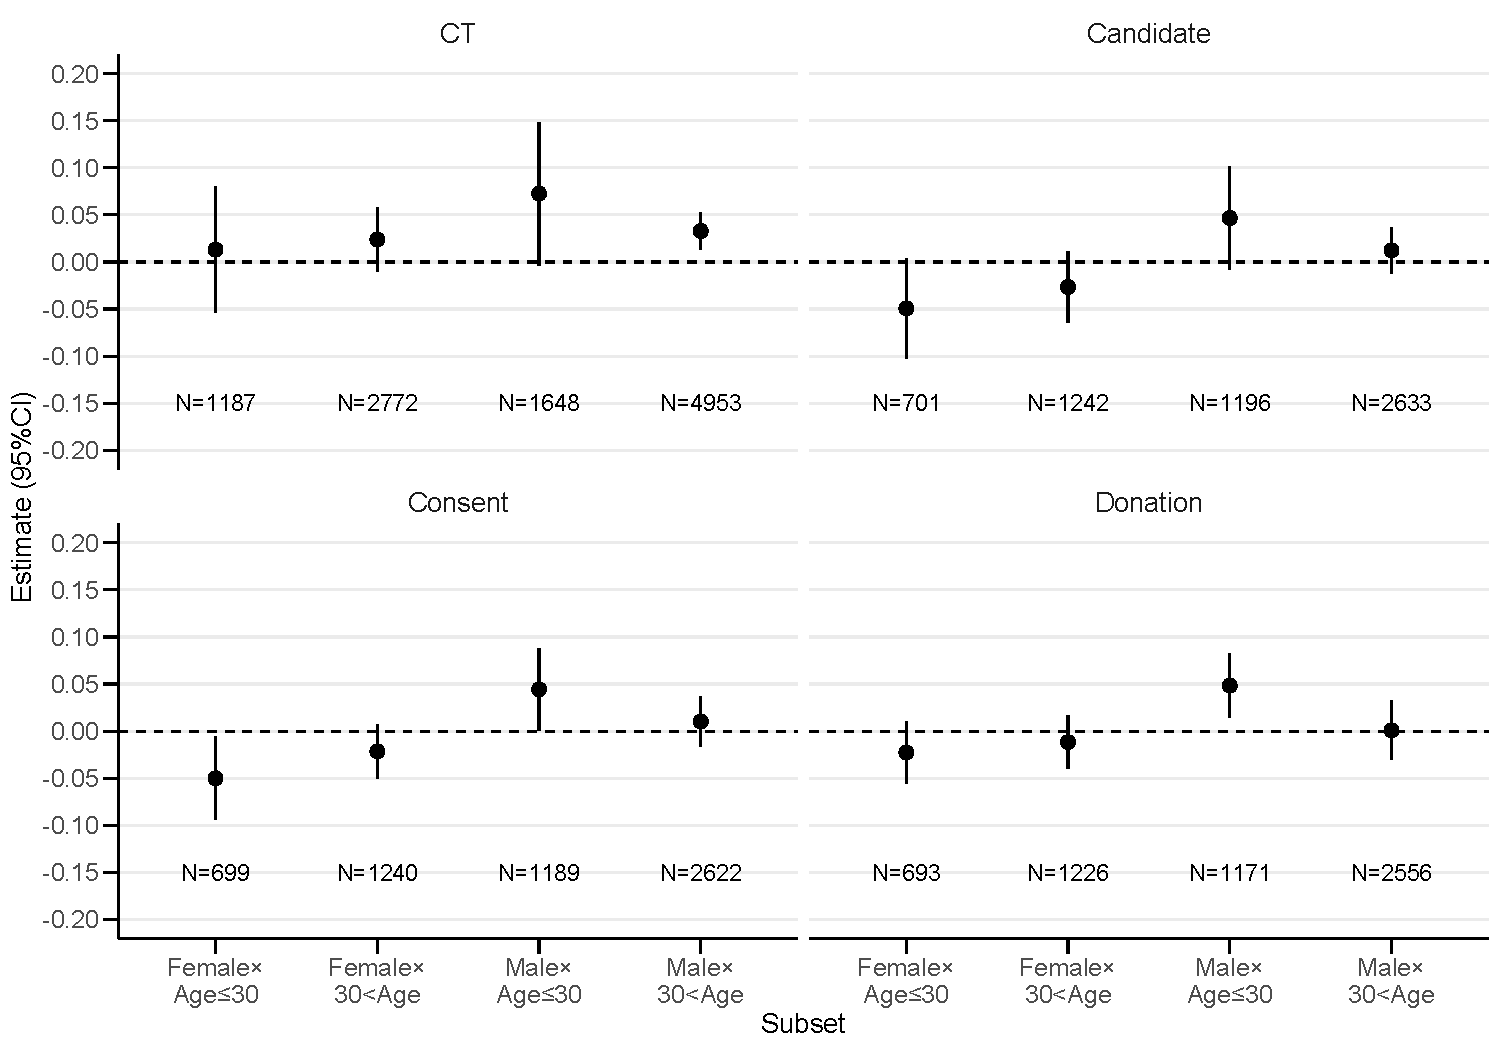
\includegraphics[width=0.75\linewidth]{C:/Users/katoo/Desktop/JMDP/RCT-Nudge/docs/slide/220818解析途中報告_files/figure-beamer/plotB-hetero-after-reply-gender-age-1} \end{center}
\end{frame}

\begin{frame}{Heterogenity by Gender x Age: Message C}
\protect\hypertarget{heterogenity-by-gender-x-age-message-c}{}
\begin{center}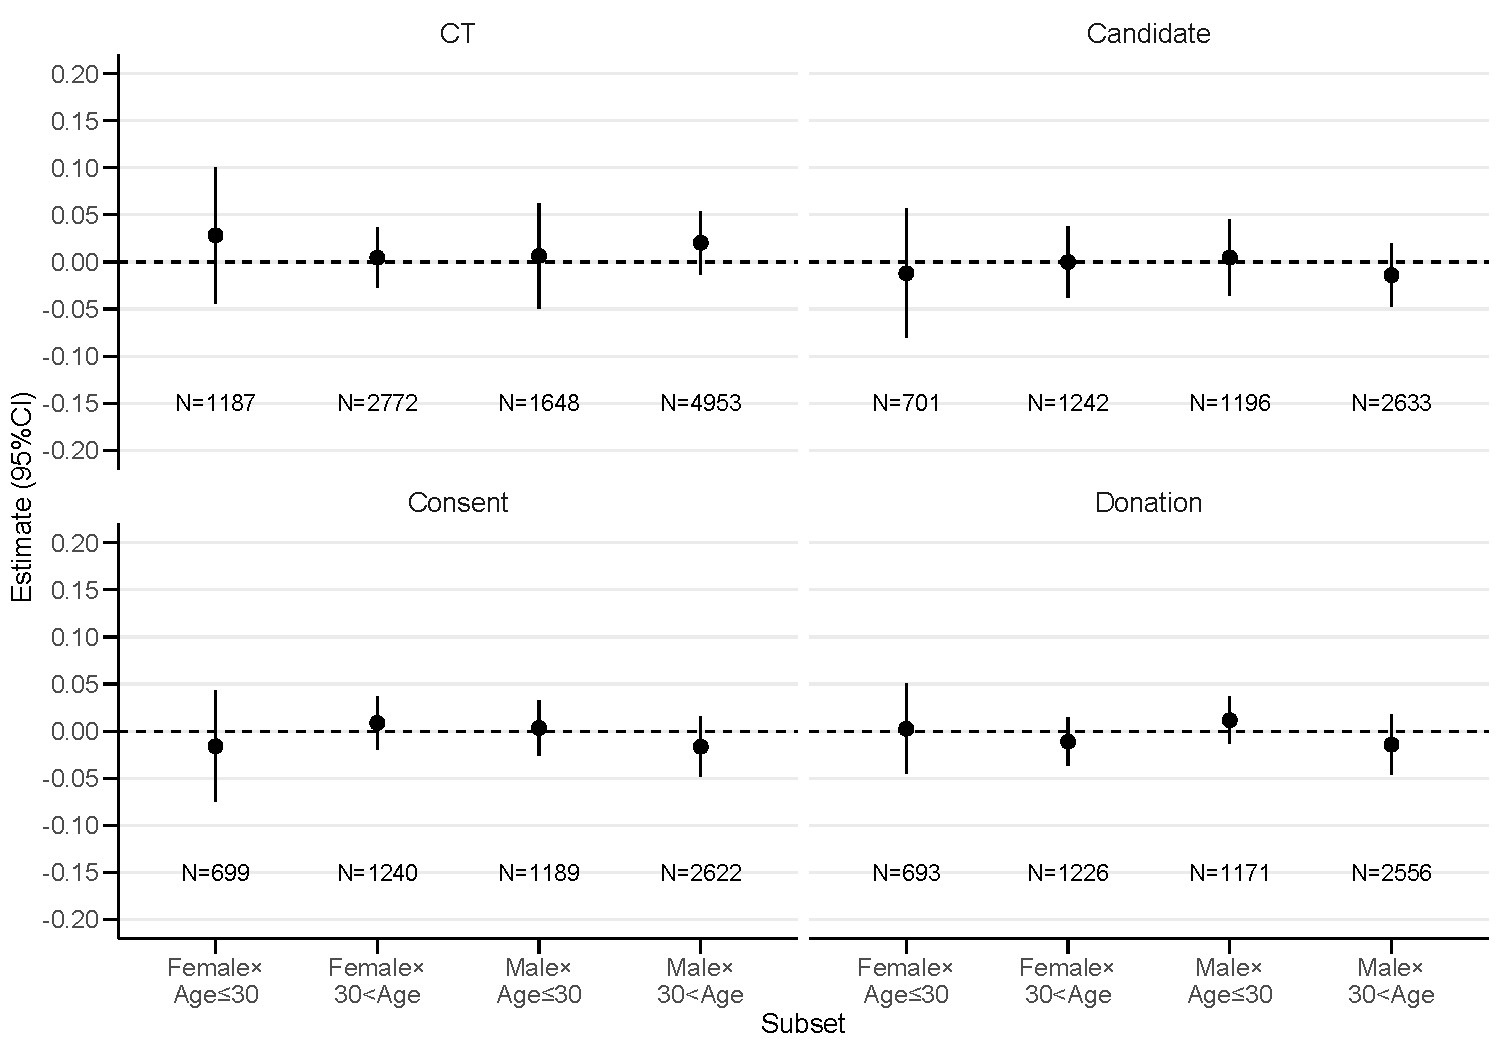
\includegraphics[width=0.75\linewidth]{C:/Users/katoo/Desktop/JMDP/RCT-Nudge/docs/slide/220818解析途中報告_files/figure-beamer/plotC-hetero-after-reply-gender-age-1} \end{center}
\end{frame}

\begin{frame}{Heterogenity by Gender x Age: Message D}
\protect\hypertarget{heterogenity-by-gender-x-age-message-d}{}
\begin{center}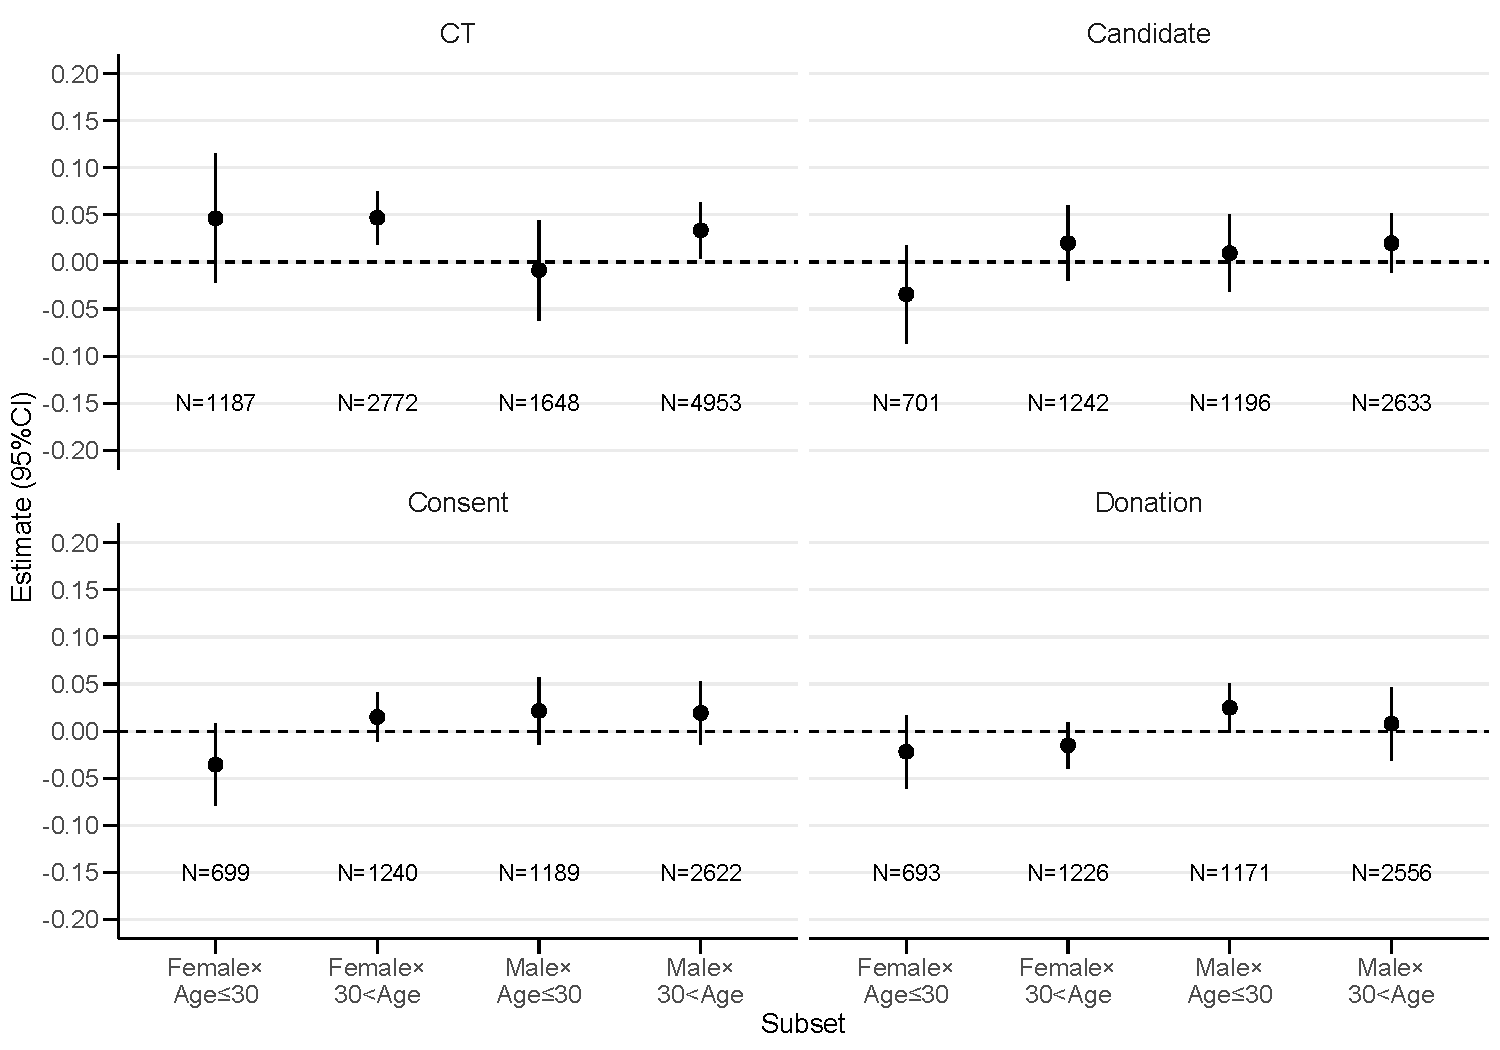
\includegraphics[width=0.75\linewidth]{C:/Users/katoo/Desktop/JMDP/RCT-Nudge/docs/slide/220818解析途中報告_files/figure-beamer/plotD-hetero-after-reply-gender-age-1} \end{center}
\end{frame}

\begin{frame}{Geographical Heterogenity}
\protect\hypertarget{geographical-heterogenity-1}{}
\begin{itemize}
\tightlist
\item
  都道府県ごとに10平方キロメートル当たりの病院数を計算し、
  0.5カ所以上ある地域とそうでない地域でサンプルを分割した

  \begin{itemize}
  \tightlist
  \item
    1カ所以上:東京・大阪
  \item
    1カ所未満:神奈川・愛知
  \end{itemize}
\item
  それぞれのサブサンプルで効果を推定する
\end{itemize}
\end{frame}

\begin{frame}{Heterogenity by Geography: Message B}
\protect\hypertarget{heterogenity-by-geography-message-b}{}
\begin{center}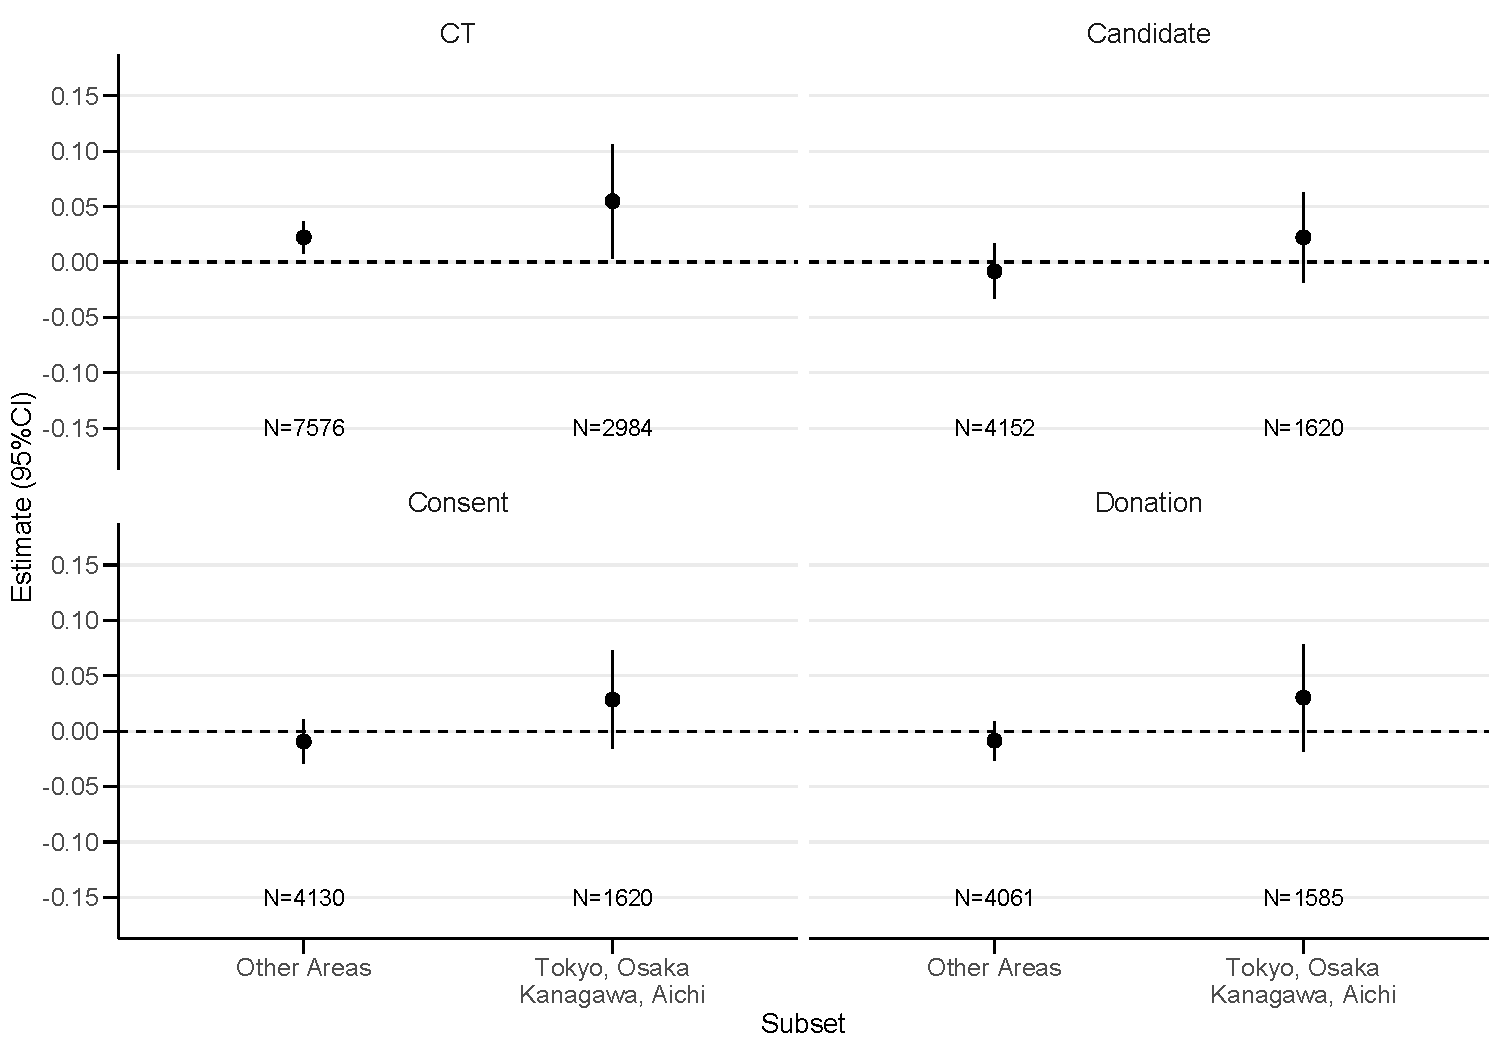
\includegraphics[width=0.75\linewidth]{C:/Users/katoo/Desktop/JMDP/RCT-Nudge/docs/slide/220818解析途中報告_files/figure-beamer/plotB-hetero-after-reply-geo-1} \end{center}
\end{frame}

\begin{frame}{Heterogenity by Geography: Message C}
\protect\hypertarget{heterogenity-by-geography-message-c}{}
\begin{center}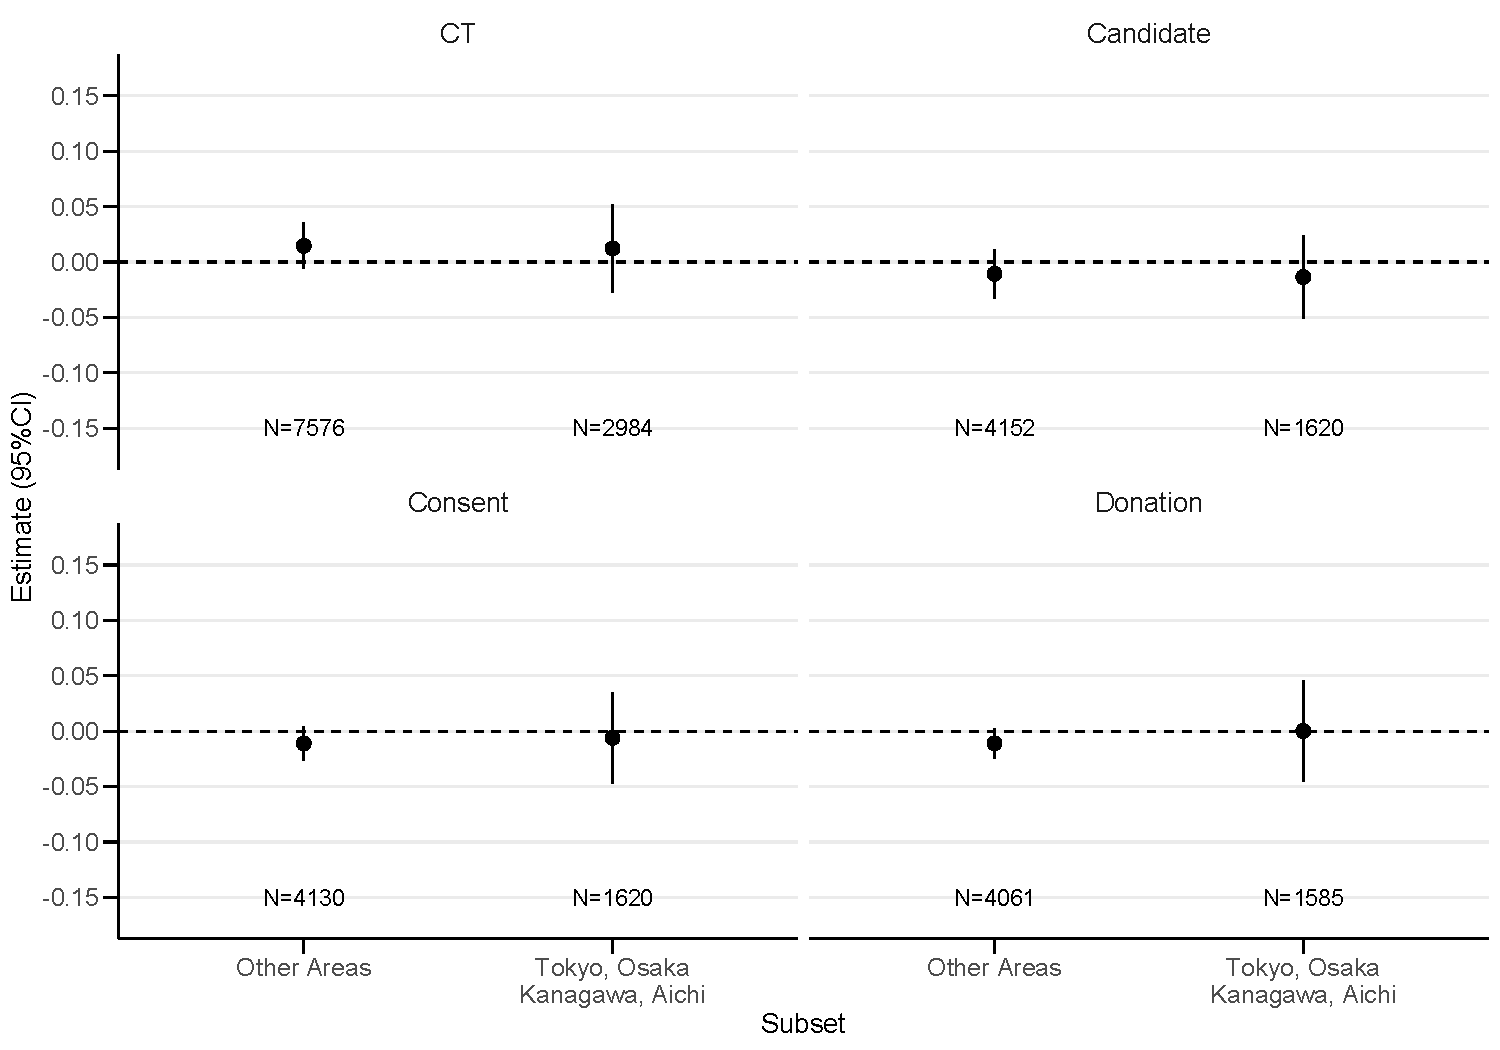
\includegraphics[width=0.75\linewidth]{C:/Users/katoo/Desktop/JMDP/RCT-Nudge/docs/slide/220818解析途中報告_files/figure-beamer/plotC-hetero-after-reply-geo-1} \end{center}
\end{frame}

\begin{frame}{Heterogenity by Geography: Message D}
\protect\hypertarget{heterogenity-by-geography-message-d}{}
\begin{center}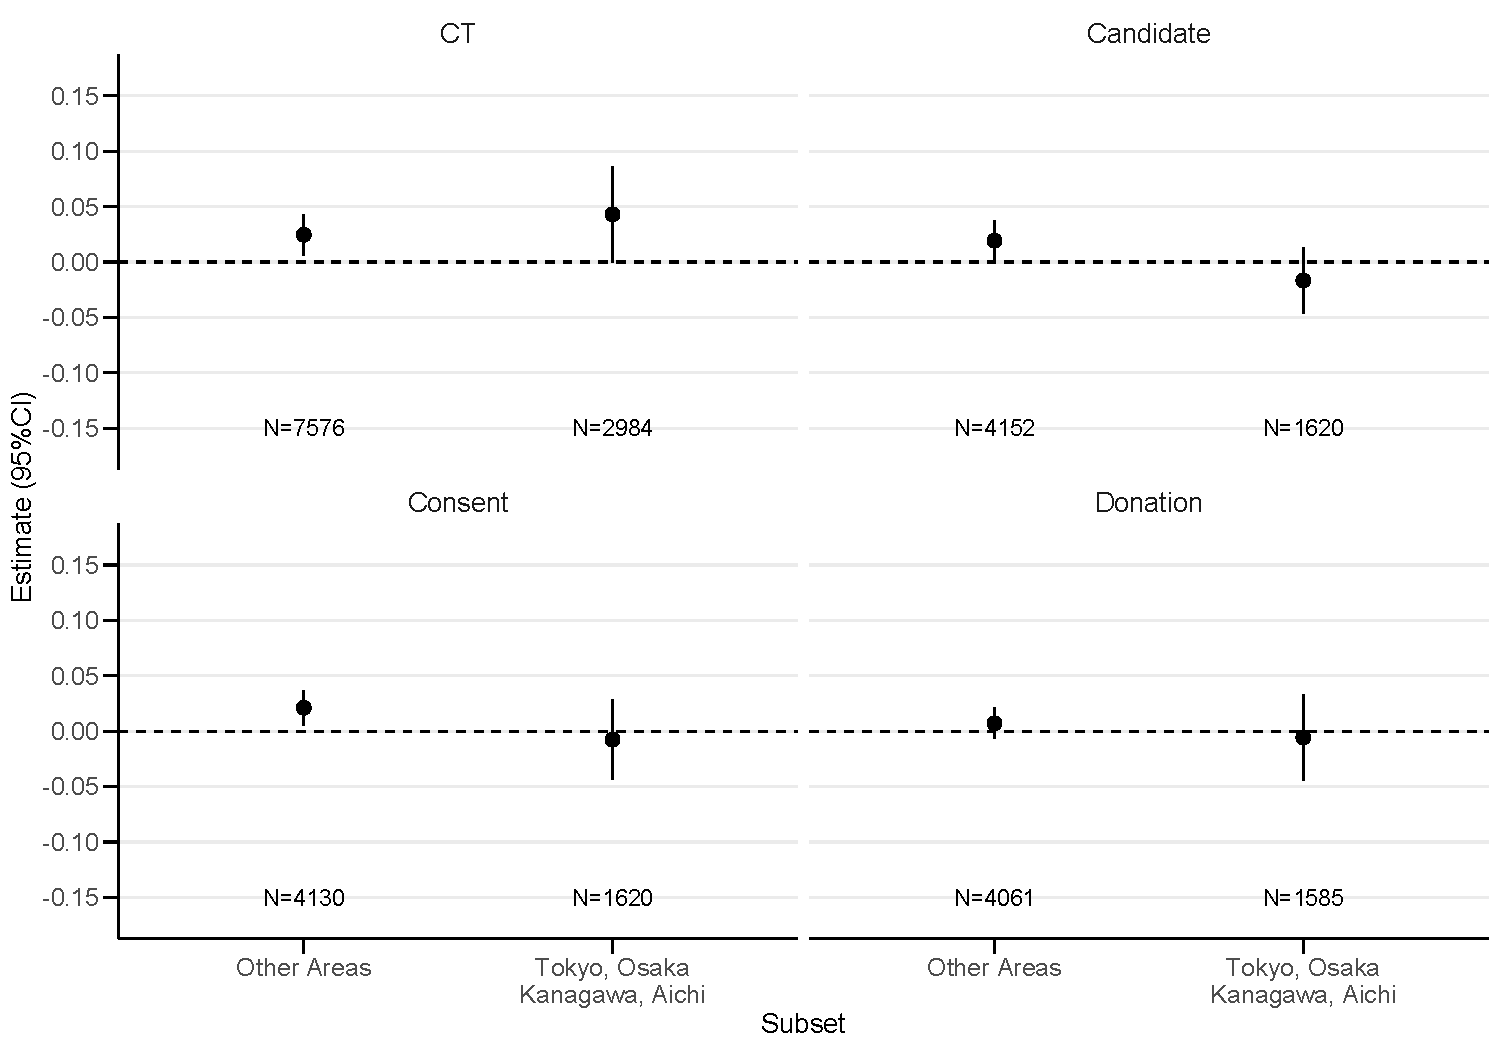
\includegraphics[width=0.75\linewidth]{C:/Users/katoo/Desktop/JMDP/RCT-Nudge/docs/slide/220818解析途中報告_files/figure-beamer/plotD-hetero-after-reply-geo-1} \end{center}
\end{frame}

\end{document}
